
\documentclass[review]{elsarticle}
\biboptions{numbers,sort&compress}
\usepackage{lineno}
\usepackage{xspace}
\usepackage[T1]{fontenc}
\usepackage{lmodern}
\modulolinenumbers[5]

\journal{Applied Energy}

%% `Elsevier LaTeX' style

%%%%%%%%%%%%%%%%%%%%%%%

%%%% packages and definitions (optional)
\usepackage{placeins}
\usepackage{changes}

%\usepackage{supertabular}
\usepackage{footnote}
%\makesavenoteenv{tabularx}
\usepackage{booktabs} % nice rules (thick lines) for tables
\usepackage{longtable} % for 'longtable' environment
\usepackage{pdflscape} % for 'landscape' environment
\usepackage{microtype} % improves typography for PDF
\usepackage{hhline}
\usepackage{amsmath}
\usepackage{pifont}
\usepackage{mathrsfs}
\usepackage{rotating}
\usepackage{tablefootnote}
\usepackage{multirow}
\usepackage{longtable}
\usepackage{enumitem}
\usepackage{mathtools}
\usepackage{amssymb}
\usepackage{float}
\usepackage{footnote}
\usepackage{slashbox}
\newcommand{\abs}[1]{\left\lvert #1 \right\rvert}
%\usepackage[singlelinecheck=false % <-- important]{caption}
%\usepackage{adjustbox}
%\usepackage{cite}
%\usepackage[demo]{graphicx}
%\usepackage{caption}
%\usepackage{subcaption}

\usepackage{booktabs}
\usepackage{threeparttable, tablefootnote}

\usepackage{tabularx}
\newcolumntype{b}{>{\hsize=1.0\hsize}X}
\newcolumntype{s}{>{\hsize=.5\hsize}X}
\newcolumntype{m}{>{\hsize=.75\hsize}X}
\newcolumntype{x}{>{\hsize=.25\hsize}X}

\graphicspath{{figures/}}

% tikz %
\usepackage{tikz}
\usepackage{chronology}
\usetikzlibrary{arrows.meta}

\usetikzlibrary{positioning, arrows, decorations, shapes, calc }
% Define block styles
\tikzstyle{decision} = [diamond, draw, fill=blue!20, 
text width=4.5em, text badly centered, node distance=3cm, inner sep=0pt]

\tikzstyle{const} = [rectangle, draw, text centered, fill=orange!20]
\tikzstyle{data} = [rectangle, draw, text centered, fill=green!20]

\tikzstyle{block} = [rectangle, draw, text centered, fill=blue!20]
\tikzstyle{line} = [draw, -latex']
\tikzstyle{cloud} = [draw, ellipse,fill=red!20, node distance=6em,
minimum height=2em]



\usetikzlibrary{shapes.multipart}
\usetikzlibrary{positioning}
% hyperref %
\usepackage[hidelinks]{hyperref}
% after hyperref %
\usepackage{cleveref}
\usepackage{datatool}
%\usepackage[nonumberlist,nopostdot,nonumberlist,acronym,toc,section]{glossaries}
\usepackage[xindy,nonumberlist]{glossaries}
\newacronym{<++>}{<++>}{<++>}
\newacronym{I$^2$CNER}{I$^2$CNER}{International Institute for Carbon Neutral Energy Research}
\newacronym{MARKAL}{MARKAL}{MARKet ALlocation}
\newacronym{TIMES}{TIMES}{The Integrated MARKAL-EFOM System}
%\newacronym[longplural={metric tons of heavy metal}]{MTHM}{MTHM}{metric ton of heavy metal}


\makeglossaries

\newcommand{\greencheck}{{\color{green}\checkmark}}
\newcommand{\xmark}{{\color{red}\ding{55}}}
\usepackage[includefoot,bottom=8pt]{geometry}



\begin{document}
\begin{frontmatter}
\title{The role of current and emerging technologies in meeting Japan's mid- to long-term carbon reduction goals}

%\date{}                     %% if you don't need date to appear

%% Authors
\author[uiuc]{Anshuman Chaube\corref{corrauthor}}
\cortext[corrauthor]{Corresponding Author}
\ead{achaube2@illinois.edu}
\author[ku]{Andrew Chapman}
\author[uiuc]{James Stubbins}
\author[uiuc]{Kathryn D. Huff} %



% Institutes of the authors
\address[uiuc]{Department of Nuclear, Plasma, and Radiological Engineering, University of Illinois at Urbana-Champaign, Urbana, IL 61801, United States}
\address[kuead]{Multiscale Science and Engineering for Energy and the Environment, International Institute for Carbon-Neutral Energy Research, Kyushu University, 744 Motooka, Nishi-ku, Fukuoka 819-0395, Japan.}
\address[kumech]{Department of Mechanical Engineering, Kyushu University,744 Motooka, Nishi-ku, Fukuoka 819-0395, Japan.}

	
\begin{keyword}
%insert keywords here
energy model \sep
Japan \sep
hydrogen fuel cell \sep
nuclear power \sep
carbon capture
\end{keyword}


\begin{abstract}

We simulated possible pathways to meeting 2030 and 2050 emission targets within the Japanese electricity supply sector using a single-region \gls{TIMES} model. Key features of our simulations include the incorporation of novel technologies, like hydrogen electrolysers, carbon capture, photochemical water splitting, and emerging photovoltaic cells, long-term impact assessment up to the year 2100, the inclusion of life-cycle emission and learning curves for technology costs and emission coefficients. Results indicate that a hybrid approach, using nuclear power and hydrogen from renewable energy-based electrolysis, is cost-effective and provides long-term emission reduction along with energy security. Nuclear, wind, solar, and hydrogen from renewables emerge as key emission reduction technologies, while natural gas with carbon capture plays a minor role.

\end{abstract}

\end{frontmatter}
%\glsresetall
\glsaddall

%\linenumbers

\printglossary[title=Abbreviations]

\section{Introduction} \label{Introduction}
In order to mitigate climate change and to improve environmental outcomes, many nations are actively seeking to reduce carbon emissions, and have formalised this goal through the Paris Agreements \cite{united_nations_framework_convention_on_climate_change_unfccc_submission_2015}. The largest contribution to global \gls{GHG} emissions, some 73\%, comes from energy consumption in the transportation, electricity and heat, buildings, manufacturing, and construction sectors \cite{ge_4_2020}. \added{Energy use in buildings in particular generates 17.5\% of all emissions \mbox{
\cite{ritchie_emissions_2021}}.} However, there is significant uncertainty surrounding these carbon-neutral energy transitions regarding the economically optimal shares and deployment rates of clean energy sources and their long-term impact on the energy system. The emergence of novel technologies like \added{high-efficiency utility-scale }  \gls{CCS} \added{(henceforth referred to as }\gls{CCS}\added{) }  and hydrogen power also raises questions about their role in \gls{GHG} mitigation and the sensitivity of the energy transition to uncertainties in these technologies' investment cost, efficiency, and carbon footprint.

We are probing these questions by simulating cost-optimised energy transitions in the electricity supply sector with rigid carbon constraints using a suite of existing and emerging electricity generation and storage technologies. We use Japan as a proxy for a developed nation committed to addressing climate change. However, the results have global significance. Like many other developed nations, Japan has been rapidly deploying renewables \deleted{and has attempted to transition away from nuclear power since the }  \added{, and in the wake of the }  Fukushima Daiichi accident \deleted{\mbox{
\cite{international_energy_agency_latest_2019}}. Yet Japan is also considering }  \added{, it shut down its nuclear reactors and increased its reliance on coal \mbox{\cite{international_energy_agency_latest_2019, noauthor_electricity_2019}}. However, now Japan is } reinvigorating its nuclear power sector, \added{as} evidenced by the restart of \added{some of} its nuclear reactors \cite{iaea_pris_nodate}. Additionally, Japan is actively developing plans to deploy hydrogen power under the Basic Hydrogen Strategy \cite{noauthor_basic_2017} and has shown interest in utilising \gls{CCS} \cite{meti_report_2020}. Therefore, due to Japan's similarity to other developed nations and its willingness to consider a variety of commercial and pre-commercial low-carbon technologies,  \deleted{lessons learnt from these decarbonisation simulations} \added{simulating likely transition pathways for decarbonisation of the Japanese electricity sector} could inform global energy policy \added{. Our simulations provide these insights} by delineating potential transition \deleted{pathways, identifying} \added{scenarios that consider multiple combinations of a variety of technological options, and our sensitivity analyses identify} key novel technologies  \deleted{,} and their most significant parameters.
%
%%Developed nations rich in natural resources can reduce \gls{GHG} emissions by switching to natural gas or implementing \gls{CCS} at fossil fuel plants. However, these options are often economically infeasible for developing nations, which will lead to increased emissions through greater coal use \cite{international_energy_agency_latest_2019}. Japan, a developed nation without fossil fuel resources, is likely to follow a different path to reduce emissions, evidenced by the restart of nuclear reactors and a shift towards large-scale renewable energy deployment .

The context of the Japanese transition strategy also captures the priorities, subtle limitations, and lack of specificity in other developed nations' energy transition plans. Although influenced by the Paris Agreements, Japanese energy policy is governed chiefly by the Basic Energy Plan \cite{noauthor_basic_2017}, which outlines national policy towards a new energy system for the years 2030 and 2050 cognizant of limited indigenous resources, the impact of the Fukushima incident, and external pressures on energy supplies \cite{meti_annual_2018}. The plan reaffirms Japanese benchmarks for evaluating the energy system, first and foremost, within the context of energy security, followed by economic efficiency, safety, and the environment (summarised as `3E+S'; ibid). Although the Japanese 3E+S goals and the Paris Agreement targets have some parallels, the plan does not detail how the 2050 emission reduction target of 80\% is to be met. Matsuo et. al have suggested that electrification of a number of sectors will be required to achieve the ambitious 2050 target, underpinned by low-carbon technologies \cite{matsuo_quantitative_2018}. For the power sector to achieve such a target, near-zero emissions are required, and early action utilising existing technologies is preferable to delayed action utilising future technologies \cite{ashina_roadmap_2012}. The strategies currently under consideration include reinvigorating nuclear power, deploying \gls{CCS} to fossil fuel power plants, and ushering in a hydrogen economy based on renewable energy-based electrolysis as well as hydrogen imports from abroad \cite{ashina_roadmap_2012, matsuo_quantitative_2018, noauthor_basic_2017}. 

This research aims to investigate the likely suite of electricity generation and storage technologies, as well as their feasibility in meeting Japan's carbon reduction goals, while being cognizant of energy policy, resource limitations, demand growth, emerging technologies, and economic constraints using the \gls{TIMES} framework. Our dynamic simulations of transition scenarios, which focus on minimising the cost of the transition while satisfying CO$_2$ emission constraints, suggest potential economically feasible decarbonisation pathways that meet the increasing near-term electricity demand. Additionally, we assess the significance of key economic parameters of emerging technologies through sensitivity analysis, in order to highlight the most impactful parameters and hence guide research and development efforts focused on these technologies.

\FloatBarrier
\section{Background and literature review} \label{litreview}
The Paris Agreement commits individual nations to significant carbon reduction over time through the \gls{INDC} mechanism \cite{united_nations_framework_convention_on_climate_change_unfccc_submission_2015}. Japan, as a signatory to the Paris Agreements, has submitted an INDC with the following goals and timelines: reduce GHG emissions by 26\% compared to 2013 levels by 2030, and reduce overall GHG emissions by 80\% or more by 2050, through the ``development and diffusion of low-carbon technologies and transition to a low-carbon socio-economic structure" \cite{united_nations_framework_convention_on_climate_change_unfccc_submission_2015}. 
Aware of these targets, many researchers have evaluated Japan's future energy system using a variety of modelling approaches, which we review below. Using the \gls{MARKAL} model, considering the uncertainties of technology development, Ozawa et al. found that hydrogen will play a major role in the future energy system, reliant on both nuclear power and \gls{CCS} to reduce electricity sector emissions to nearly zero by 2050 \cite{ozawa_hydrogen_2018}. Recognising the benefits that renewable energy will play in reducing carbon emissions, and the issues of intermittency of renewables, Li et al. explored the role of hydrogen as a storage medium through power-to-gas approaches in Kyushu, Japan. Their study identified that power-to-gas can increase the effective utilisation rate of renewable energy, and the use of hydrogen in the gas network, effectively pairing the electricity and gas networks, overcomes current renewable electricity curtailment issues \cite{li_potential_2019}. Cognizant of the Japanese government's strategic approach to carbon reduction out to 2050 via energy system reform, Chapman and Pambudi also identify a strong role for nuclear, renewables, and hydrogen under a carbon constrained, optimal cost MARKAL/TIMES simulation approach \cite{chapman_strategic_2018}. Considering Japan's economic conditions and demographic trends, such as moderate GDP growth and rapid population ageing, Kuriyama et al. suggest that 2030 targets can be met or exceeded (with up to 42\% GHG reduction) with limited renewable energy growth and a 15\% contribution from nuclear, or without nuclear, under a renewable growth scenario \cite{kuriyama_can_2019}. However, these trends and energy system changes will likely be insufficient to meet the more ambitious 2050 targets. 

Taking a more holistic view in line with the Japanese government's 3E+S targets, ambitious research and development to enable high levels of renewable deployment is necessary to not only meet deep emission reduction goals, but to also reduce Japanese dependence on imported fuels, which would affect both CCS and nuclear deployment rates into the future. Consensus on policy options and priorities also has a large influence on modelling outcomes for the Low Carbon Navigator, which assesses Japanese energy and emission options out to 2050 \cite{moinuddin_japan_2019}. A seminal work by Sugiyama et al. harmonises a number of modelling approaches for Japan's long-term (up to 2050) climate change mitigation options, utilising national and global general and partial equilibrium models \cite{sugiyama_japans_2019}. Model results are contrasted under six scenarios which incorporate a baseline, a range of emissions reductions (50-80\%), and regional obligations for global models (ibid.) under the Paris Agreement target of an 80\% reduction. Each of the models assessed recognise the importance of renewable energy deployment by 2050, notably hydro, solar, and wind, with varying contributions from nuclear energy and fossil fuels, predominantly natural gas. Additionally, for Japan, the option of importing carbon-free hydrogen was identified as potentially playing a critical role \cite{akimoto_estimates_2010, matsuo_global_2013, oshiro_diffusion_2015, sugiyama_japans_2019}. Many studies consider hydrogen a critical part of Japan's low-carbon energy transition, as it can improve energy security, it can be produced from multiple sources, and lacks emissions from fuel combustion \cite{iida_hydrogen_2019}. Global modelling efforts consider the incorporation of long-distance international transport of hydrogen with end uses dominated by passenger and freight fuel cell vehicles and power generation, via both mixed and direct combustion. Electricity from hydrogen is estimated to emerge in Japan from 2030 onwards, as nuclear and coal-fired power generation reduce towards 2050 \cite{ishimoto_significance_2017}. From a policy standpoint, Japan has committed to achieving a hydrogen society, with the primary goal of cost parity of hydrogen with competing fuels, which requires a three-fold reduction in cost by 2030 and further reductions into the future \cite{nagashima_japans_2018}. Under the Basic Hydrogen Strategy, the Japanese government aims to realise low cost hydrogen use in power generation, mobility, and industry, develop international supply chains to ensure stable supply, expand renewable deployment, revitalise regional areas, and develop hydrogen related technologies \cite{noauthor_basic_2017}. The strategy aims to account for both economic and geopolitical impacts and the need to prioritise research and development to overcome the economic and technical challenges \cite{nagashima_japans_2018}. A common thread across previous research is the uncertainty surrounding \gls{CCS}, particularly with regard to scaling up and public acceptance issues, and the role that nuclear energy will play, largely due to policy reform which occurred after the Fukushima nuclear accident \cite{oshiro_mid-century_2019}.

The model and the approach proposed in this research uniquely build on the modelling consensus outlined in the literature review and expand the consideration of technologies by including emerging near-term alternatives, and potentially disruptive technologies post-2050. This work leverages the dynamic simulation capabilities of \gls{TIMES} \cite{loulou_etsap-tiam:_2008} by incorporating learning curves for parameters such as investment and \gls{OM} costs, efficiency, and emission coefficients. Our model incorporates not only direct emissions, but also lifecycle emissions of all conventional and emerging technologies, the latter of which is an often neglected externality. This enables a more meaningful analysis of the global warming potential of emerging technologies, as life-cycle emissions become significant when considering deep emission reductions of the order of 80\% from current levels. By modelling the Japanese electricity supply system out to the year 2100, our aim is to detail the mid- to long-term impacts of technological development and market penetration, and to identify the suite of technologies which could underpin the successful achievement of carbon reduction.

\FloatBarrier
\section{Methodology} \label{method}
% what is TIMES
\subsection{TIMES Model Description}
\gls{TIMES} models dynamic energy systems and simulates transition scenarios as a mixed-integer linear optimisation problem that is subject to a primary objective function and additional constraints
\cite{loulou_etsap-tiam:_2008} . The generation, refinement, supply, storage, and trade of energy commodities are modelled across multiple sectors and multiple regions using a wide variety of in-built commodity and process types. Emissions can be associated with energy commodities or processes as an emission coefficient per unit commodity produced or consumed. 

%basic features of model
We outline salient features of our model in this section, while the data used for our simulations are in \ref{Appendix}. The relevant input files can be accessed online \cite{chaube_arfci2cner_2021}. The objective function in our single-region model is the overall cost of the transition. The major constraints in our simulations are the demand for electricity (Table \ref{demand}), emission constraints on the electricity-generation sector based on Japan's \gls{INDC} (Table \ref{co2-limits}), and feasible nameplate capacity deployment limits (Table \ref{caplim}). Miscellaneous assumptions are summarised in Table \ref{misc-assump}. In summary, our model minimises the transition cost while meeting the increasing electricity demand and achieving the required emission cuts using a combination of generation and storage technologies. 

\begin{table}[H]
\centering
	\caption{Electricity demand increase over the simulation time frame. \added{The demand for 2017-2030 is obtained from \mbox{
\cite{noauthor_electricity_2019}}
, the rest of the curve is based on estimated population growth trends.} }
	\vspace{0.1in}
	\begin{tabularx}{0.4\textwidth}{p{0.15\textwidth} p{0.25\textwidth}}
		\hline
\textbf{Year} & \textbf{Annual demand} \\
 & \textbf{increase} \\
\hline
2017-2030 & 1.7 \% \deleted{\mbox{
\cite{noauthor_electricity_2019} }
} \\
2031-2050 & 1.0 \% \\
2051-2070 & 0.5 \% \\
2070-2100 & 0.0 \% \\
\hline 
	\end{tabularx}
\label{demand}
\end{table}

\begin{table}[H]
\centering
	\caption{Emission constraints.}
	\vspace{0.1in}
	\begin{tabularx}{0.6\textwidth}{p{0.05\textwidth} p{0.2\textwidth}p{0.05\textwidth} p{0.3\textwidth}}
		\hline
\textbf{Year} & \textbf{Emission limit} & \textbf{Base} & \textbf{Reduction} \\
 & & \textbf{year} & \textbf{from base year} \\
\hline
2030 & 438 Mt CO$_2$-eq. & 2013 & 26 \% \\
2050 & 75 Mt CO$_2$-eq. & 1990 & 80 \% \\
2100 & 75 Mt CO$_2$-eq. & 2050 & 0 \% \\
\hline 
	\end{tabularx}
\label{co2-limits}
\end{table}

While Japanese electricity demand is expected to grow in the near future  \cite{noauthor_electricity_2019}, long-term electricity demand in Japan is expected to plateau, or even decrease, due to Japan's ageing population. However, precisely quantifying this rate of decrease is challenging, as this reduction in population will likely be accompanied by increased electrification of transportation and industrial sectors. Hence, post-2030, we have assumed a demand curve based on increased electrification driving increasing demand, which eventually plateaus due to the aforementioned expected demographic changes. The model captures the initial condition of the post-Fukushima Japanese electricity supply system using \added{historical data} The Energy Data and Modelling Centre's data from 2013-2016 \cite{the_institute_of_energy_economics_japan_energy_2018}. Long term impacts of factors such as the retirement of the existing nuclear reactor fleet and the deployment of emerging technology is assessed by simulating the system until 2100. Using \gls{TIMES} day-night and seasonal time periods
\cite{loulou_etsap-tiam:_2008}, the daily and seasonal variability of renewables is incorporated. The availability of renewables varies during these time periods based on the annually averaged capacity factors of renewables in Japan\mbox{\cite{the_institute_of_energy_economics_japan_energy_2018, irena_renewable_2020}}.

We account for the carbon cost of each technology using an emission coefficient that incorporates both direct emissions and life cycle emissions averaged over the entire operating lifetime for each technology. Using day-night and seasonal time periods\cite{loulou_etsap-tiam:_2008}, the daily and seasonal variability of renewables is incorporated. The availability of renewables varies during these time periods based on the annually averaged capacity factors of renewables in Japan \mbox{\cite{the_institute_of_energy_economics_japan_energy_2018, irena_renewable_2020}}. \added{The emission coefficient data and their sources are listed in Table \ref{eco}. The emission coefficients vary dynamically for technologies that have projections available in literature, and are linearly interpolated between available data points until the last available projection, beyond which they are held constant. For hydrogen fuel cells and electrolysers, emission coefficients vary in magnitude across different technologies but the learning curves follow similar trajectories due to the similarity of technologies \mbox{\cite{iea_technology_2015} } \mbox{\cite{pinaud_technical_2013}}. The lifecycle emissions for \gls{PWS} are unknown, hence we have assumed them to be the same as that of \glspl{SOEC} as both are lab-scale technologies with similar deployment time-frames, and \gls{PWS} must have similar or lower life-cycle emissions as \gls{SOEC} to be competitive}.

%scenario description
To explore possible pathways to curbing \gls{GHG} emissions, we simulated five transition scenarios of varying likelihoods, with different sets of technologies enabled for deployment, as described in Table \ref{scen-table}. The first set includes conventional technologies such as  \gls{USC}, \gls{lng}, solar photovoltaic, wind energy (with onshore, offshore-fixed, and offshore-floating considered separately), and utility-scale lithium-ion battery storage. New deployments of oil-fuelled power plants are disabled due to the declining use of oil for electricity generation in accordance with Japan's goal of energy security and independence, as per the Basic Energy Plan. The second set of technologies considered includes emerging carbon-neutral technologies that are already commercialised or close to commercialisation, namely emerging solar photovoltaic (modelled as a composite of perovskites and CdTe solar cells), \gls{CCS}, and utility-scale hydrogen power. For hydrogen power, steam reforming, steam reforming with \gls{CCS}, \glspl{AEC}, \glspl{PEMEC}, \glspl{PEMFC}, and \glspl{SOFC} were incoporated based on their technological potential. Along with these two technology groups, we also explore the potential impact of nuclear energy. Nuclear power has significant advantages over renewables including long operational lifetimes, extremely low life-cycle emissions, and high capacity factors. However, nuclear power faces extremely low public acceptance in Japan after the Fukushima-Daiichi accident, therefore its future in Japan is highly uncertain. Hence, transition scenarios with and without new nuclear reactor deployment must be juxtaposed to assess the importance of the role of nuclear in emission reduction. Finally, the long-term impact of nascent hydrogen technologies on the hydrogen economy is assessed in an additional scenario. In this scenario, the potential commercialisation of \gls{SOEC} and \gls{PWS} post-2050 is explored in the absence of new nuclear power.

\begin{table}[H]
\centering
	\caption{Electricity supply transition scenario definition based on enabled technologies.}
	\vspace{0.1in}
	\begin{tabularx}{0.65\textwidth}{p{0.1\textwidth} p{0.18\textwidth} p{0.15\textwidth} p{0.18\textwidth}}
\hline 
\textbf{Scenario}& \textbf{Emerging} & \textbf{New} & \textbf{Nascent}\\
 & \textbf{tech.} & \textbf{nuclear} & \textbf{tech.}\\

%                 & \textbf{enabled} & \textbf{enabled} & \textbf{enabled}\\
                  \hline
%1               &   \xmark       &      \xmark     &   \xmark     \\ 
%2               &   \xmark       &      \greencheck     &   \xmark     \\ 
%3               &   \greencheck       &      \xmark     &   \xmark     \\ 
%4               &   \greencheck       &      \greencheck     &   \xmark     \\ 
%5               &   \greencheck       &      \xmark     &   \greencheck     \\ 
1               &  No       &         No     &     No  \\ 
2               &   No       &      Yes     &     No  \\ 
3               &   Yes     &         No      &     No   \\
4               &   Yes     &      Yes     &     No  \\ 
5               &   Yes     &      No     &     Yes  \\ 
\hline
	\end{tabularx}
\label{scen-table}
\end{table}


%misc assumptions
Exogenous variables such as economic data, emission coefficients, nameplate capacity limits, and growth rates are detailed in Tables \ref{eco}, \ref{caplim}, and \ref{growrate} respectively. Prices and projections for fossil fuels and nuclear fuel are incorporated \cite{wittenstein_projected_2015, world_bank_commodity_2016, international_energy_agency_world_2019}. Learning curves for costs and life-cycle emissions are compiled from existing data (Table \ref{eco}) based on expected scaling of manufacturing, availability of manufacturing materials, and the use of clean energy for manufacturing energy system components. These learning curves are modelled as piecewise linear functions interpolated between the available data points, with the curve plateauing at the latest value for a given parameter, as detailed in Table \ref{eco}. Capacity limits of renewables and \gls{PWS} are based on their land-use requirements. The maximum annual capacity growth rates for existing technologies are held constant. The growth rate of nuclear power is based on historic trends and current pressure vessel manufacturing limitations \cite{iaea_pris_nodate}. The reactor size assumed in this study is 1165 MWe, based on Watts-Bar Unit 2 \cite{iaea_pris_nodate-1}. Due to a projected increase in the share of renewables, nuclear power plants must be able to load-follow to a certain extent, which is approximated in our model based on French reactors' range of capacity factors. The growth rates of all emerging technologies are modelled on the rates observed for solar photovoltaic technology, with rapid initial growth followed by gradual reduction, eventually reaching a moderate maximum attainable growth rate. One notable exception is the maximum growth rate of emerging solar technologies, which we have assumed to be the same as that of existing solar photovoltaic technologies. We assume that these technologies, some of which are already commercialised or close to commercialisation, will benefit immensely from the already streamlined solar photovoltaic manufacturing and supply chain. Therefore, they could be deployed as rapidly as conventional solar photovoltaic cells. 

All hydrogen storage devices are operated with a maximum availability factor of 90\%, making them extremely flexible for load-following. Long-term storage of hydrogen is also available using hydrogen tanks with appropriate loss factors \cite{iea_technology_2015}. For hydrogen electrolysers and fuel cells, life-cycle emissions from just the stack are considered \added{(see Table \ref{eco})} , as balance-of-plant emissions from utility scale hydrogen depend strongly on the type of plant and the source of energy used for electrolysis. Our assumptions about the reduction in the investment costs and life-cycle emissions of batteries are conservative due to the rising cost of cobalt and nickel, and lithium-ion battery manufacturing being concentrated in high \gls{GHG}-emitting nations, respectively \cite{oliveira_environmental_2015,emilsson_lithium-ion_2019,turcheniuk_ten_2018,simon_potential_2015}.

\subsection{Sensitivity analysis}
%approach, goal, what are we hoping to learn
%variables, sampling approach, median, range, which variables, which base case scenario, why
While the aforementioned scenarios identify potential pathways that are likely to result in deep emission cuts, many parameters, such as the investment cost, life cycle emissions, and lifetimes, are highly uncertain for novel technologies like \gls{CCS} and hydrogen generation and conversion technologies. Therefore, our sensitivity analysis is focused on investigating the impact of such parameters (Table \ref{sa-vars}). We analyse the sensitivity of the share of each of these technologies in the electricity-generation mix and of the system transition cost with respect to these variables.

\begin{table}[H]
\centering
	\caption{Candidate parameters and their variation in our sensitivity analysis.}
	\vspace{0.1in}
	\begin{tabularx}{0.9\textwidth}{p{0.3\textwidth} p{0.15\textwidth} p{0.15\textwidth}p{0.3\textwidth}}
\hline 
\textbf{Technology}  & \textbf{Sampled} & \textbf{Distribution}& \textbf{Distribution}\\
\textbf{Parameter} & \textbf{Distribution} & \textbf{Mean}& \textbf{Range}\\
\hline
\gls{PWS} Investment Cost       & Gaussian    & 3088 \$/kW & $\pm$20\%. \\                  
\gls{SOEC} Investment Cost      & Gaussian    & 1388 \$/kW & $\pm$20\%.\\                  
\gls{PEMEC} Investment Cost     & Gaussian    & 3800 \$/kW & $\pm$20\%.\\                  
\gls{SOFC} Investment Cost      & Gaussian    & 7399 \$/kW & $\pm$20\%.\\                  
\gls{PEMFC} Investment Cost     & Gaussian    & 7399 \$/kW & $\pm$20\%.\\                  
\gls{CCS} Gas Investment Cost   & Gaussian    & 2626 \$/kW & $\pm$20\%.\\                  
\gls{CCS} Coal Investment Cost  & Gaussian    & 5252 \$/kW & $\pm$20\%.\\
\gls{PWS} Emission Coefficient  & Triangular  & 1.08 g/kWh & 0.2-5.405 g/kWh. \\                  
\gls{SOEC} Emission Coefficient & Triangular  & 1.08 g/kWh & 0.2-5.405 g/kWh. \\
\gls{PWS} Efficiency            & Triangular  & 0.525 & 0.5-0.58. \\                               
\hline
	\end{tabularx}
\label{sa-vars}
\end{table}

While there is significant uncertainty in the investment cost of nuclear power plants \cite{lovering_historical_2016}, it varies for individual plants and not for the technology as a whole. Preliminary simulations also demonstrated that nuclear power dominates the energy mix, and its share is fairly insensitive to perturbations over known ranges of investment costs \cite{lovering_historical_2016} due to its low life cycle emissions. Consequently, we eliminated nuclear power's investment cost as a candidate for sensitivity analysis. Furthermore, Japan has been exploring low-emission alternatives to nuclear since the Fukushima Daiichi disaster. In order to assess these potential alternatives which would otherwise be eliminated from the energy mix if new nuclear reactors were deployed, we chose Scenario 5 (Table \ref{scen-table}) as our base scenario for sensitivity analysis. Ten model parameters were sampled 30 times from appropriate distributions (Table \ref{sa-vars}). The parameter value at the first year of deployment (Table \ref{eco}) was varied, but the parameter's learning curve was held constant throughout all scenarios. For example, a 20\% change in the deployment year (2030) investment cost of \gls{SOFC}s with respect to the base case scenario reduces their investment cost in 2050 by 20\% as well. This makes learning-based cost-reductions proportionate across all sensitivity analysis runs. These parameters were randomly co-varied in 30 simulations. The share of each electricity generation technology (as the ratio of cumulative technology output to the cumulative electricity demand) and output of hydrogen technologies was plotted versus each varying parameter to correlate the effect of these parameters with the penetration of these technologies into the mix. A similar approach was also used to correlate these parameters with the system's transition cost.
\FloatBarrier
\section{Results} \label{Results-and-discussion}

\subsection{Transition Scenarios}

The transition simulations' results are shown in Figures \ref{scen1}-\ref{scen5}, and summarised in Table \ref{tab:results_summary} (see Table \ref{scen-table} for scenario definitions). \added{Note that the years 2013-2016 represent the initial condition modelled using historical data \mbox{
\cite{the_institute_of_energy_economics_japan_energy_2018}}
, and the simulation results begin from 2017 onwards. } The results of each scenario are reported as annually aggregated plots of (i) the electricity that is directly supplied to the end user, (ii) the active nameplate capacities of generation and storage technologies, and (iii) the resulting emissions (direct and life cycle) from each technology. The first plot of each scenario shows a large degree of variation as generated electricity is diverted from multiple sources to storage technologies instead of being supplied directly to the end user. The output of some technologies also varies due to their ability to load-follow. The second plot describes the transitions in terms of capacities, highlighting the effect of the capacity factor of intermittent versus base-load technologies. The third plot details the sources of direct and averaged life-cycle emissions from each source.

\begin{table}[H]
\centering
	\caption{Summary of decarbonisation simulations' results.}
	\vspace{0.1in}
	\begin{tabularx}{0.9\textwidth}{p{0.1\textwidth} p{0.2\textwidth}p{0.1\textwidth}p{0.1\textwidth}p{0.1\textwidth}p{0.2\textwidth}}
		\hline
\textbf{Scenario} & \textbf{Enabled} & \textbf{Meets} & \textbf{Meets} & \textbf{Emissions} & \textbf{Cost} \\
 & \textbf{Technologies} & \textbf{2030} & \textbf{2050} & \textbf{between} & (USD) \\
 &  & \textbf{emission} & \textbf{emission} & \textbf{2050-} &  \\
 &  & \textbf{goals} & \textbf{goals} & \textbf{2100} &  \\
\hline
1 & Conventional tech., no new nuclear & Yes & No & +25 Mt & 3.51 trillion. \\
2 & Conventional tech., with new nuclear & Yes & Yes & -12 Mt & 2.66 trillion. \\
3 & Emerging tech., no new nuclear & Yes & Yes & No change & 3.19 trillion. \\
4 & Emerging tech., with new nuclear & Yes & Yes & -32 Mt & 2.80 trillion. \\
5 & Nascent tech., no new nuclear & Yes & Yes & No change & 3.18 trillion. \\
\hline 
	\end{tabularx}
\label{tab:results_summary}
\end{table}

In Scenario 1 (Figure \ref{scen1}), the model is able to meet 2030 emission goals but fails to achieve the 2050 target by a margin of 25 Mt. Emissions continue to increase by another 25 Mt by 2100, primarily due to life cycle emissions from lithium-ion storage. As in all other scenarios, coal and oil must be retired by 2030. Natural gas sees rapid growth in the near-term, but complete retirement by 2055. Once deep emission cuts have been achieved, new natural gas is deployed again from 2071 onwards for its load-following capabilities. All existing nuclear power plants must be restarted by 2022 at full operating capacity. With renewable energy as the only option for decarbonisation, significant investments in solar, onshore wind, offshore wind (both fixed-bottom and floating), and lithium-ion storage are necessary. The presence of a large share of renewables results in significant overgeneration of electricity during some years. The amount of electricity diverted to storage technologies over the entire simulation time frame is 46,342 TWh, primarily from solar (36\%), onshore wind (22\%), fixed-bottom offshore wind (22\%),and floating offshore wind (12\%). The total cost of this transition is \deleted{\textbf{3.51 trillion USD}}
 \added{3.51 trillion USD}.

\begin{figure}[H] 
\centering
%\vspace*{-3cm}
%\hspace{-3cm}
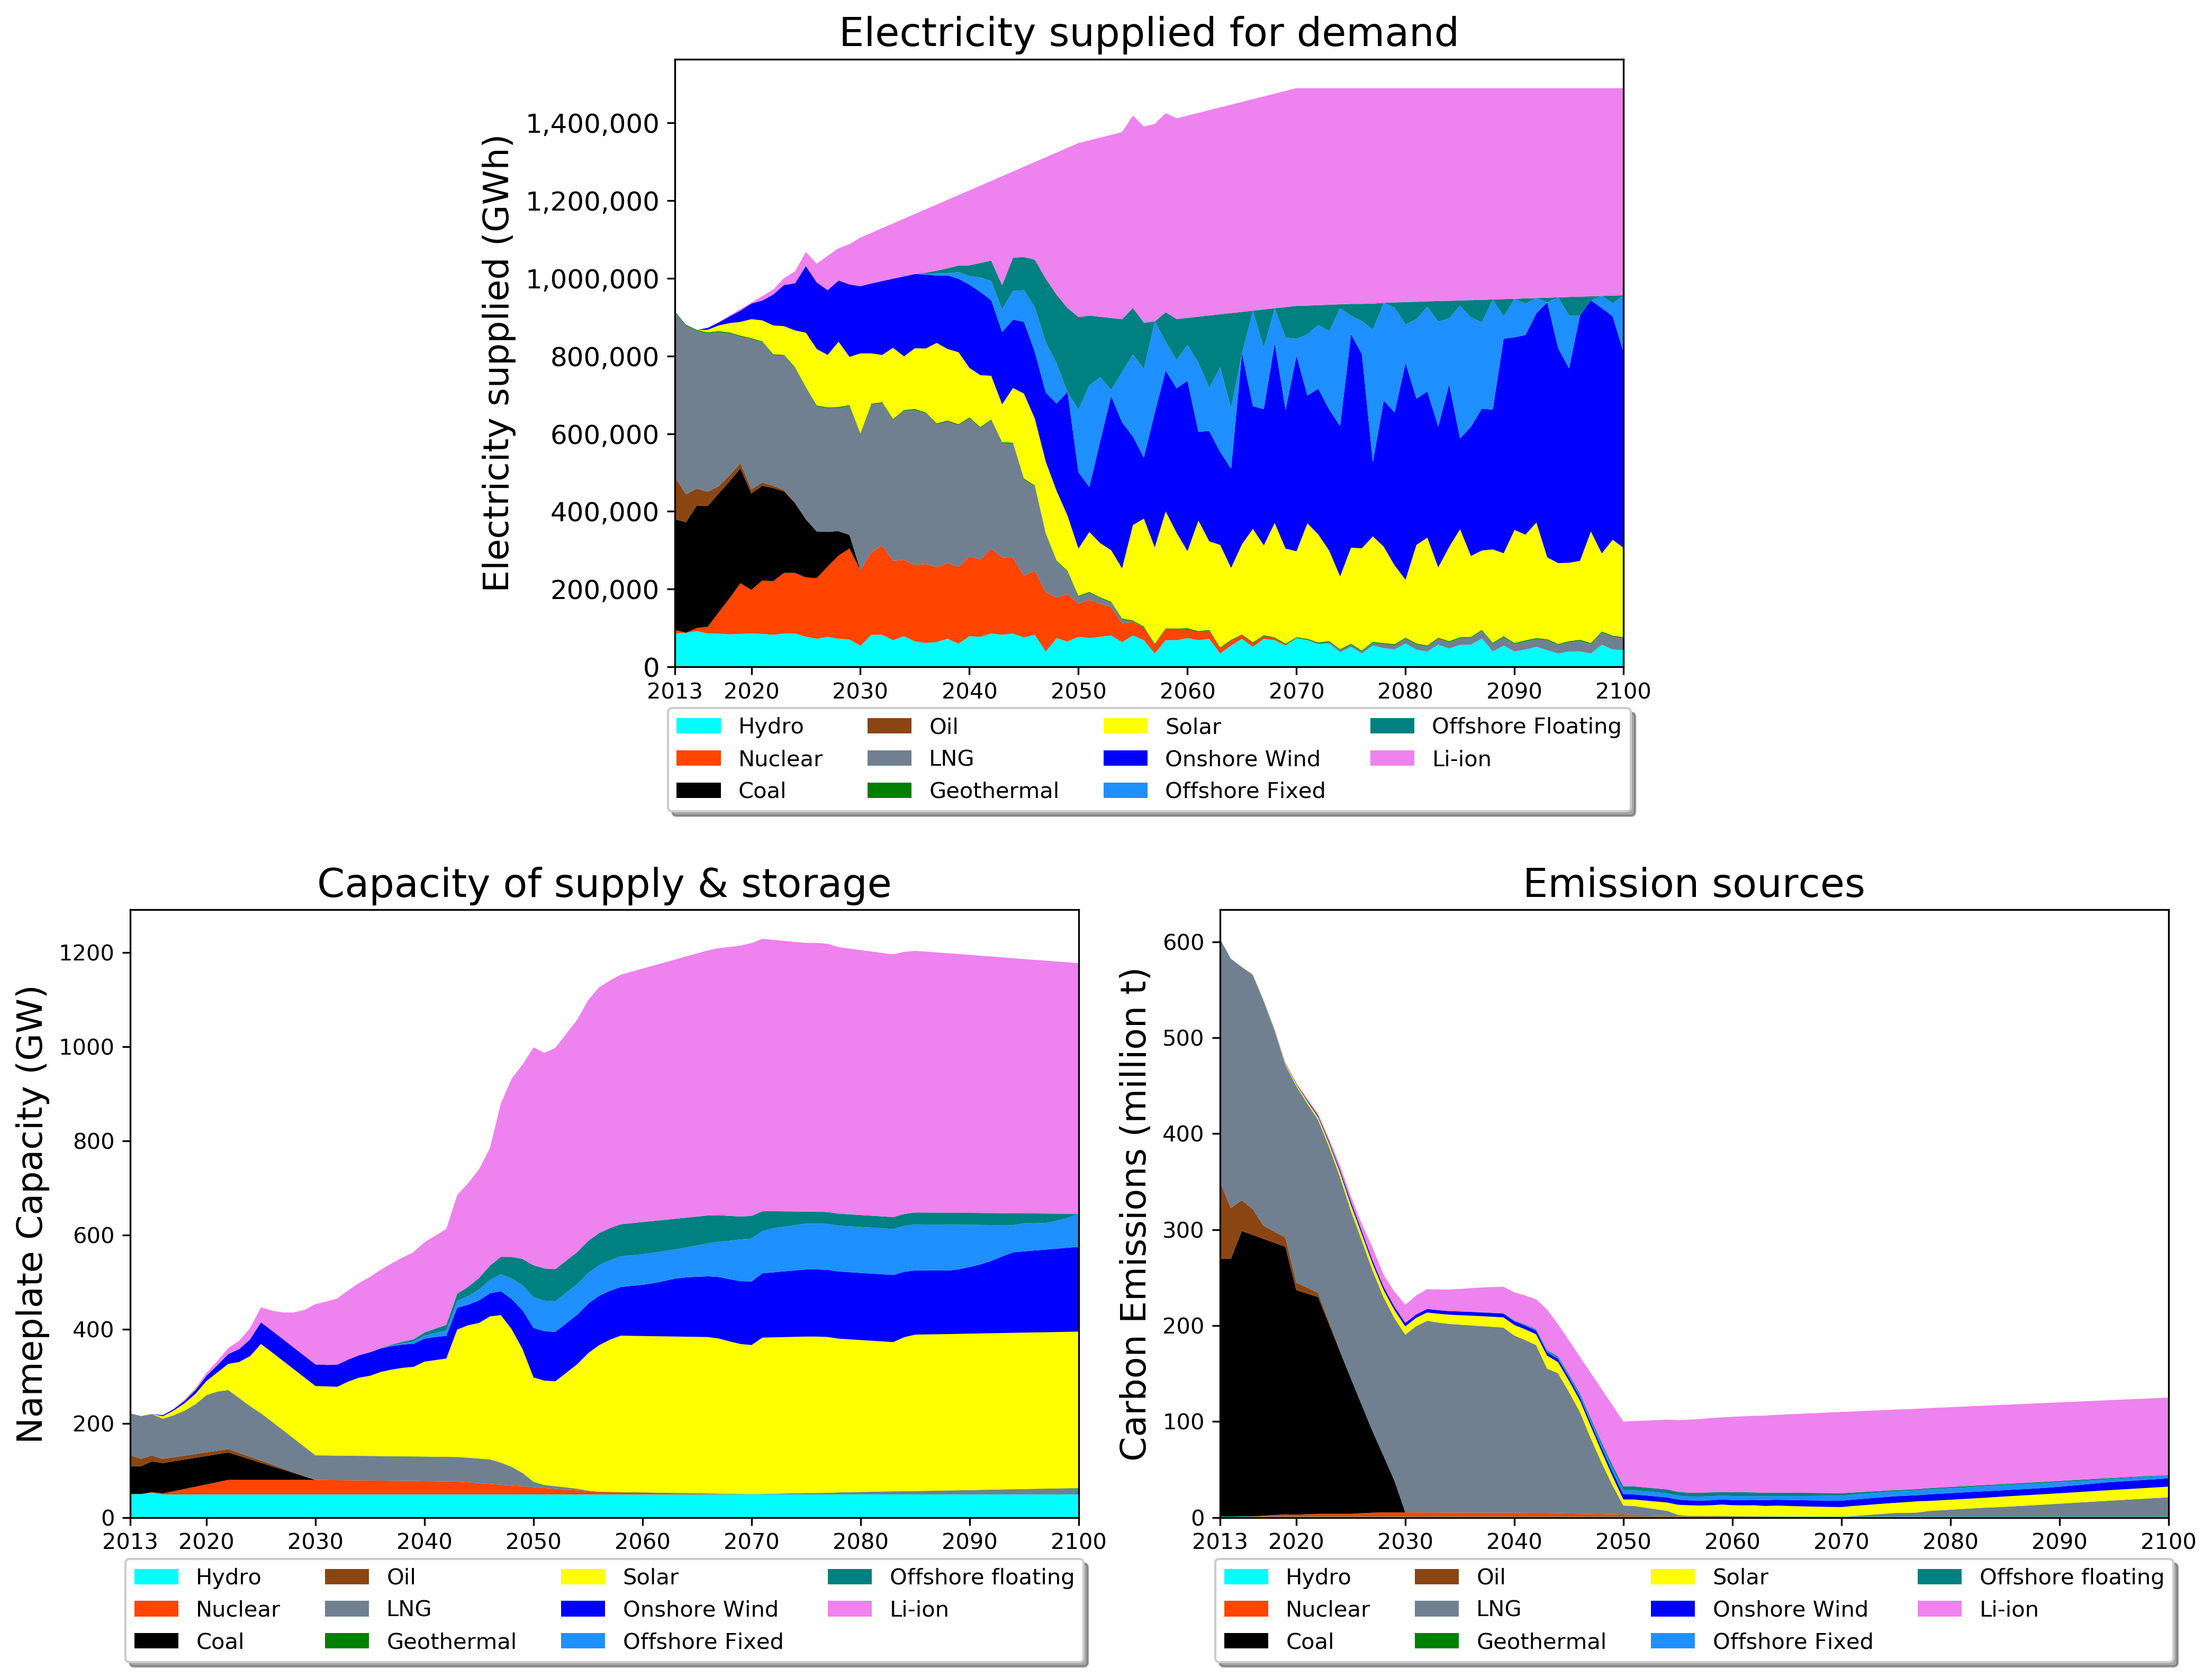
\includegraphics[scale=0.5]{figures/conv_nonuc}
\caption{Scenario 1 results (conventional technologies without new nuclear). The plot at the top shows the electricity generation mix used to meet the demand, the bottom-left figure shows the nameplate capacities of electricity generation and storage technologies that are deployed to meet the demand, and the bottom-right figure shows the sources of emission(direct and life cycle) resulting from this energy mix.}
\label{scen1}
\end{figure}

With the availability of new nuclear reactors in Scenario 2 (Figure \ref{scen2}), both 2030 and 2050 emission targets are achieved, and a further emission reduction of 12 Mt occurs by 2100. The model chooses to rapidly deploy nuclear power plants at the maximum allowed growth rate despite the high investment cost of nuclear due to its low life-cycle emissions. This nuclear-driven reduction in emissions allows natural gas power plants to operate until 2100. The share of renewables deployed during this transition reduces dramatically. This, combined with the load-following capabilities of natural gas plants and nuclear reactors, drastically decreases the capacity of lithium-ion storage deployed. 12,220 TWh of electricity is diverted to storage, primarily from nuclear (46\%), solar (41\%), and onshore wind (8\%). The total transition cost of this scenario is the lowest, at \deleted{\textbf{2.66 trillion USD.}} \added{2.66 trillion USD.} 

\begin{figure}[H] 
\centering
%\vspace*{-3cm}
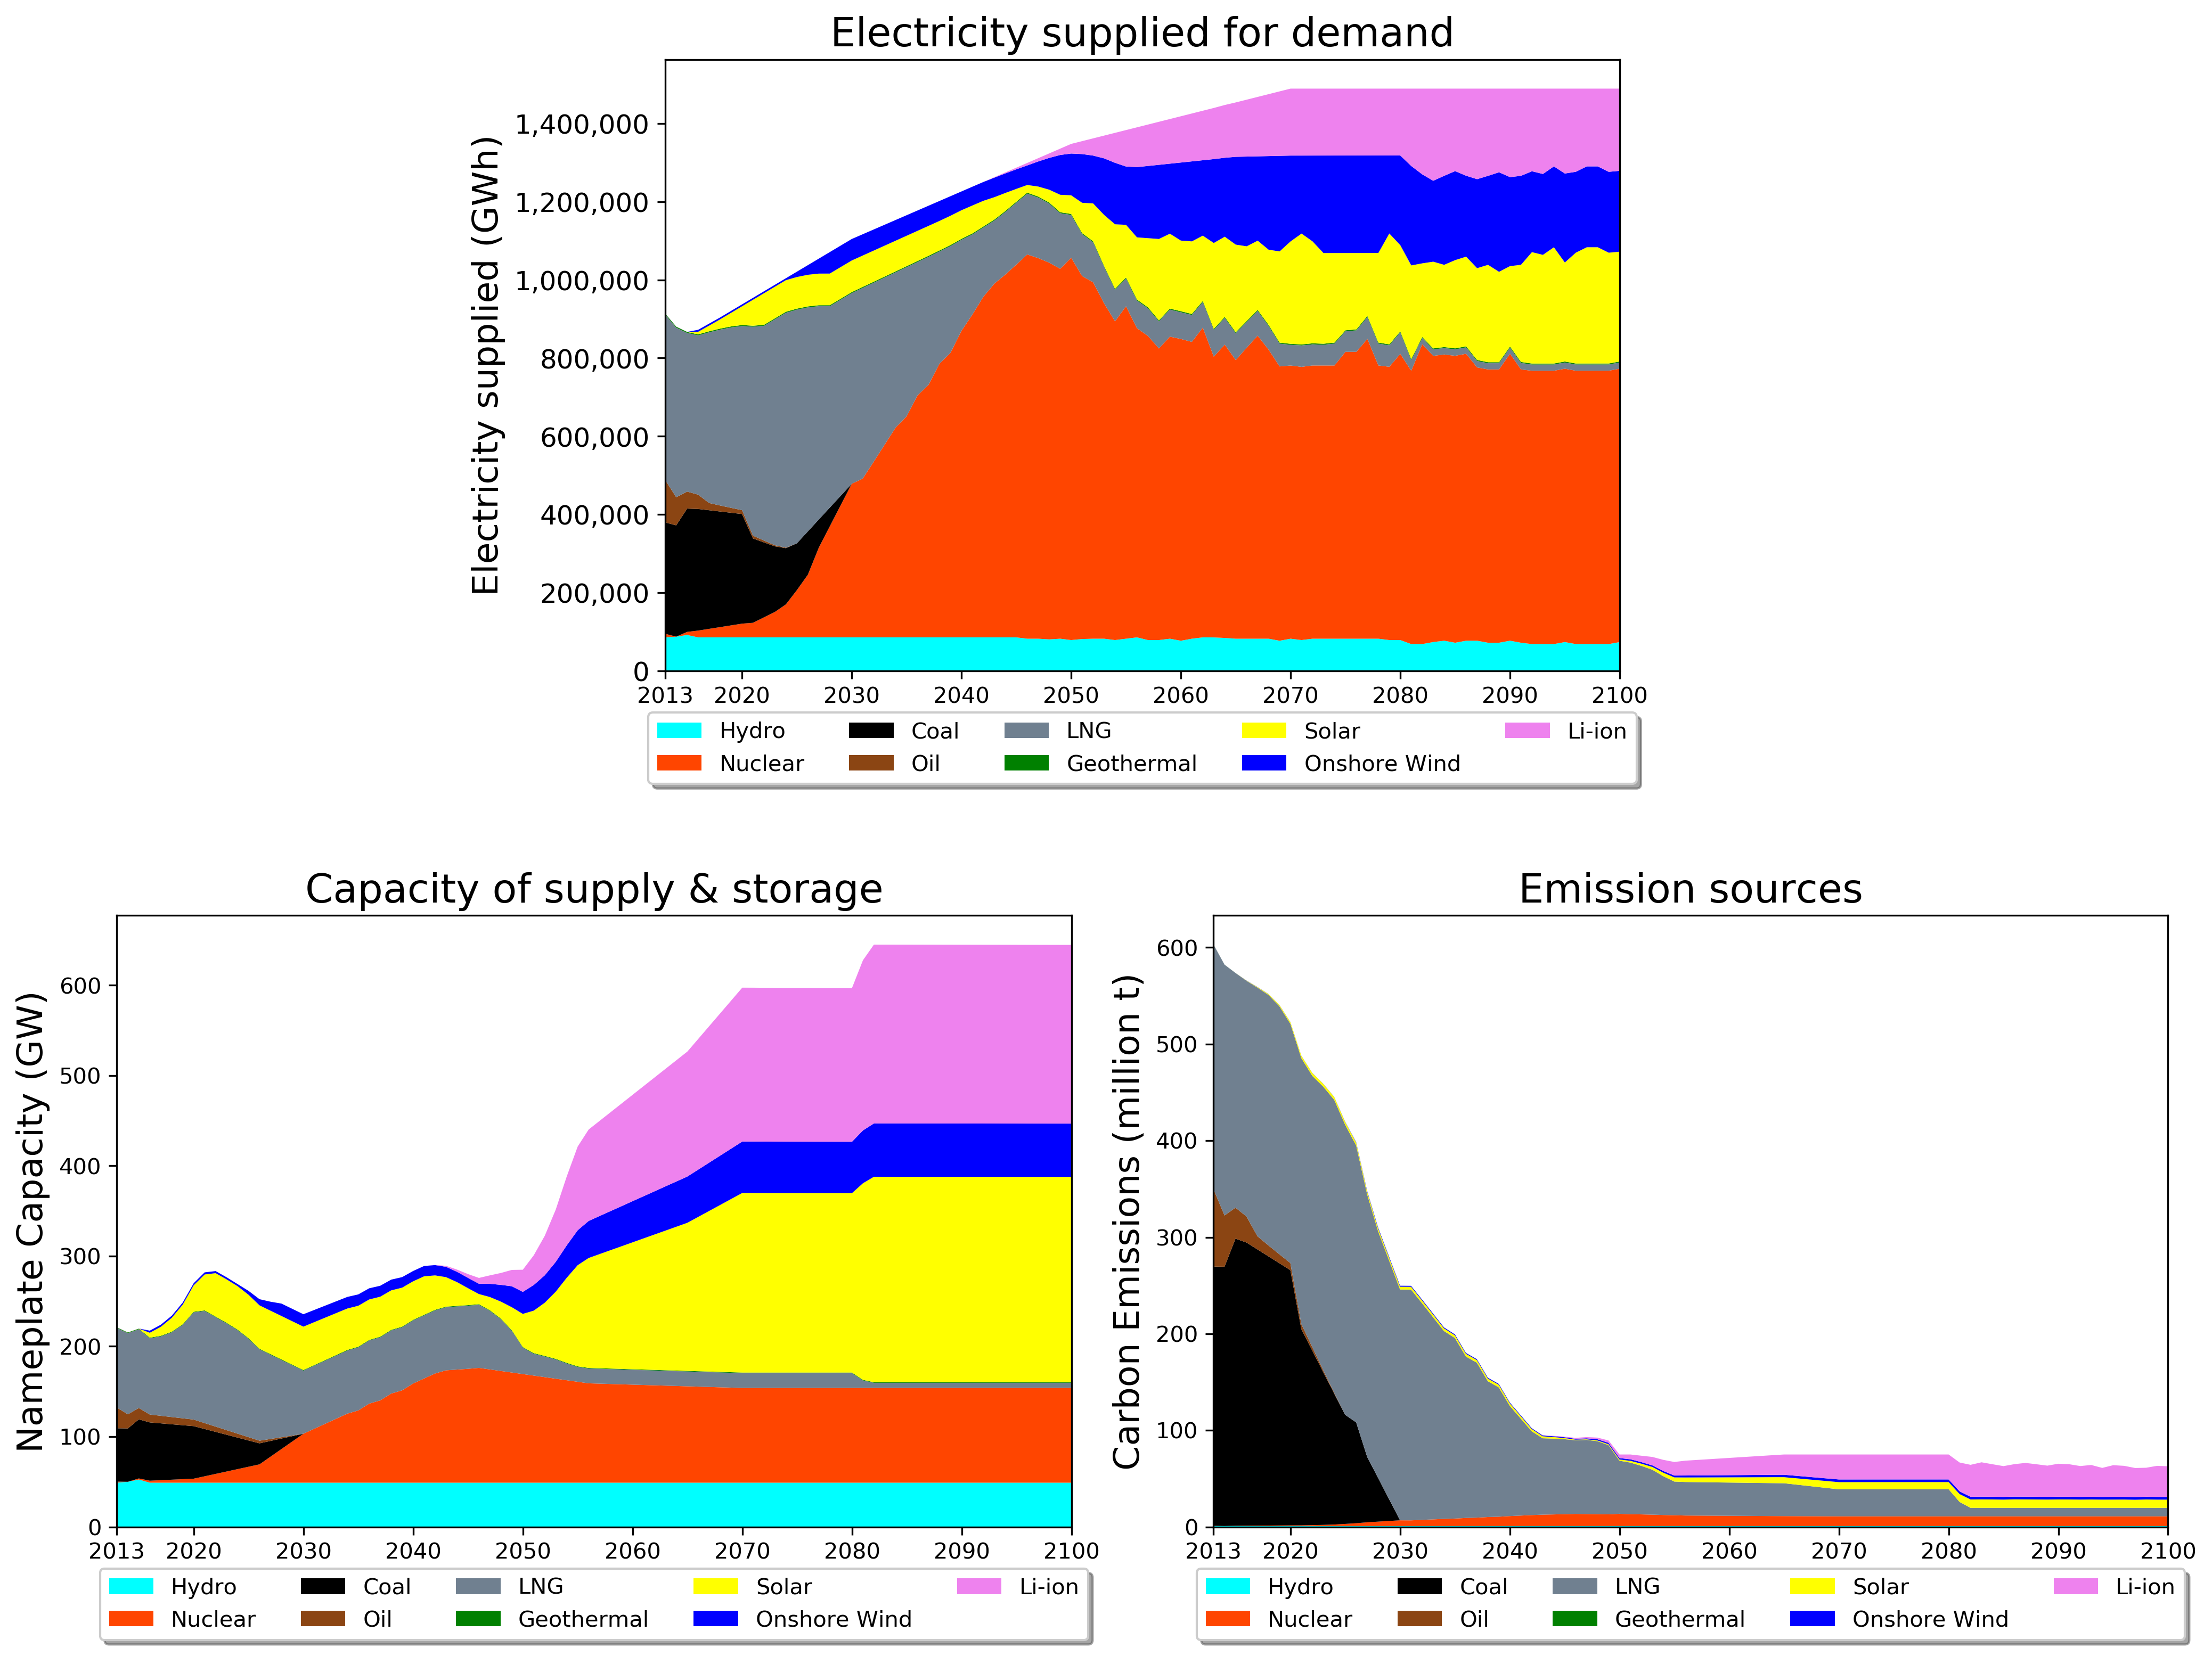
\includegraphics[scale=0.5]{figures/conv_nuc}
\caption{Scenario 2 results (conventional technologies with new nuclear). The plot at the top shows the electricity generation mix used to meet the demand, the bottom-left figure shows the nameplate capacities of electricity generation and storage technologies that are deployed to meet the demand, and the bottom-right figure shows the sources of emission(direct and life cycle) resulting from this energy mix.}
\label{scen2}
\end{figure}

Using emerging technologies without new nuclear power (Figure \ref{scen3}), the model is able to meet both the 2030 and 2050 emission reduction goals, but no further decarbonisation occurs after 2050. The results highlight the need to restart Japan's existing nuclear power plants at full capacity by 2030 in such a scenario. The deep emission cuts achieved through renewables, hydrogen, and \gls{CCS} allow the model to keep using \gls{lng} until 2100. Expansion of solar and onshore wind, along with a modest deployment of lithium-ion batteries and natural gas with \gls{CCS}, helps the model meet 2030 emission goals. After that, the model relies primarily on renewables and hydrogen to curb emissions. Rapid investment in hydrogen storage from 2030 onwards allows effective utilisation of renewables and precludes investment in offshore floating wind power. \gls{lng}-based \gls{CCS} plays a modest role as an intermediate technology before the model can complete the transition to utility-scale hydrogen. Between 2032-2077, the model generates 2,328 TWh  of electricity from \gls{CCS} technology, which is 2\% of the electricity generated over the entire simulation time frame. This results in 872 Mt of CO$_2$ being captured, which is well within the estimated 156 Gt CO$_2$ reservoir limit for Japan \cite{kato_energy_2016}. As the existing photovoltaic technology approaches the end of its lifetime and emerging solar technologies become cheaper and more efficient, they rapidly replace existing solar power, benefiting from the existing solar manufacture and supply chains. A total of 43,879 TWh of generated electricity is diverted to storage, primarily from solar and emerging solar technologies (48\%), fixed bottom offshore wind (28\%), and onshore wind (20\%). Much of this is used to generate 35,478 TWh worth of hydrogen, initially from alkaline electrolysis(1\%), but rapidly transitioning to PEM electrolysis (99\%) due to its greater efficiency and increasing cost-effectiveness. The cost of this transition is \deleted{{3.19 trillion USD}} \added{3.19 trillion USD}.

\begin{figure}[H] 
\centering
%\vspace*{-3cm}
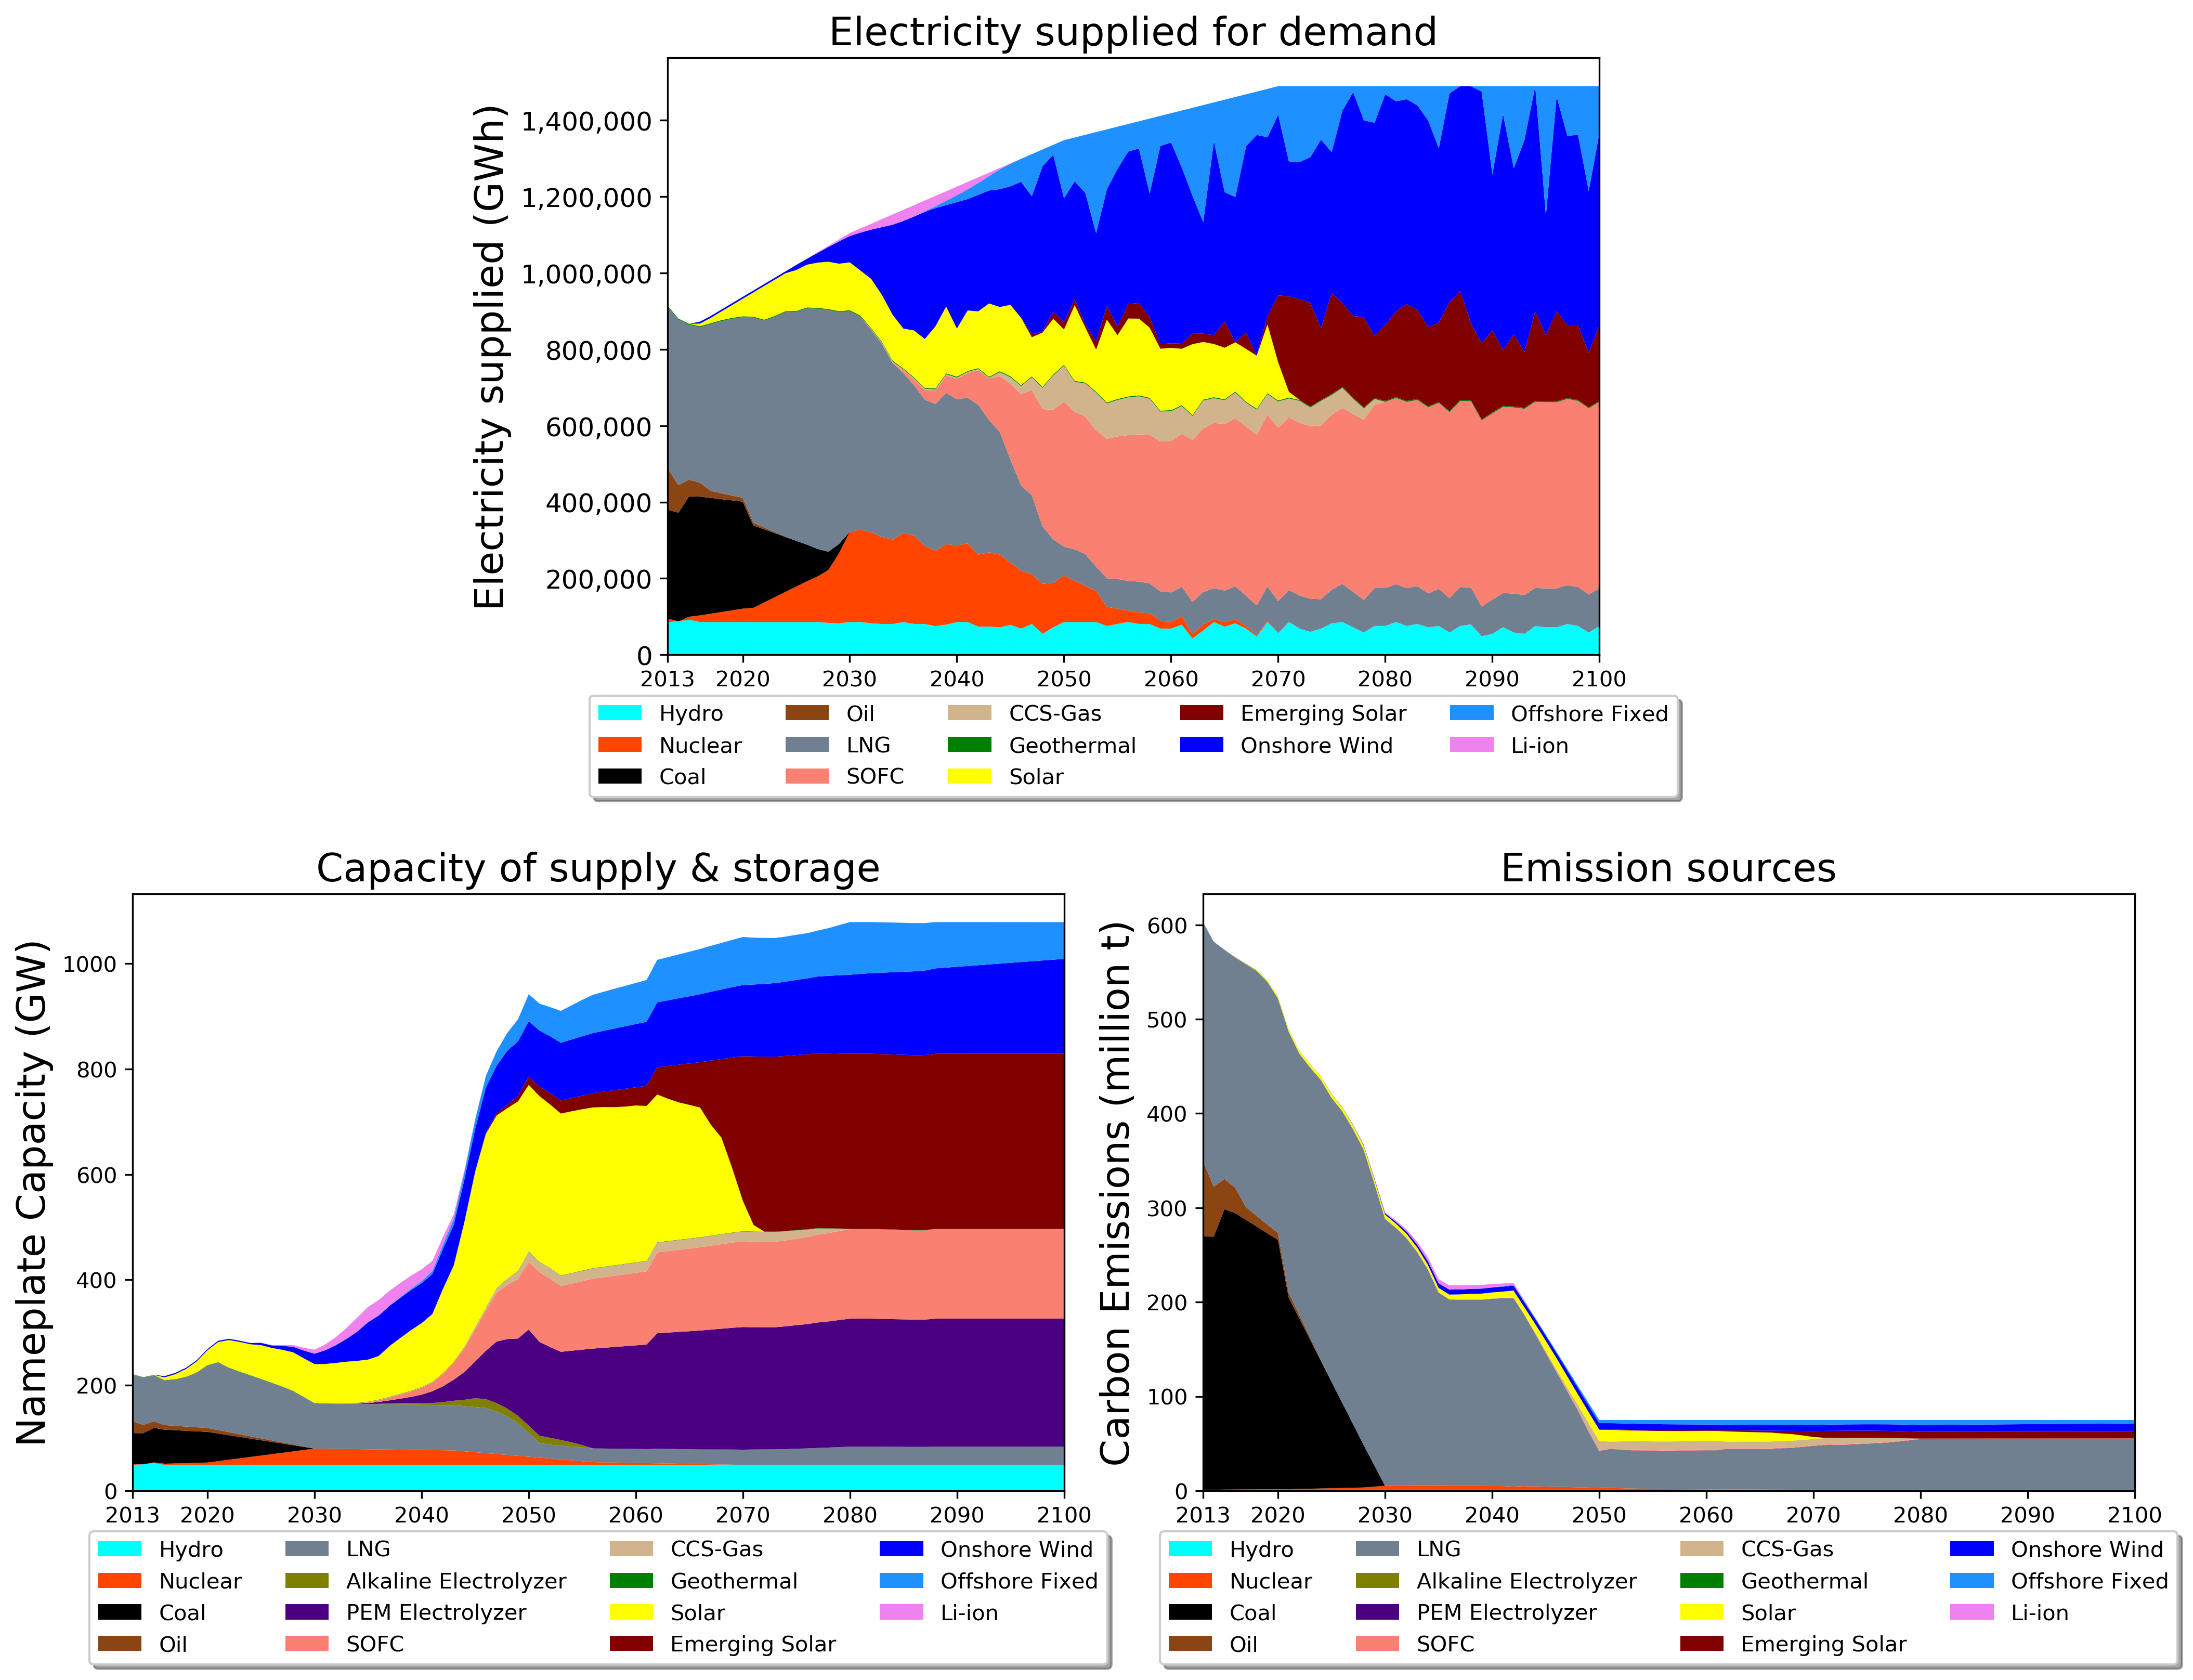
\includegraphics[scale=0.5]{figures/newtechs_nonuc}
\caption{Scenario 3 results (emerging technologies without new nuclear). The plot at the top shows the electricity generation mix used to meet the demand, the bottom-left figure shows the nameplate capacities of electricity generation and storage technologies that are deployed to meet the demand, and the bottom-right figure shows the sources of emission(direct and life cycle) resulting from this energy mix.}
\label{scen3}
\end{figure}

Deploying both emerging technologies with new nuclear reactors (Figure \ref{scen4}) results in rapid decarbonisation. Both 2030 and 2050 emission targets are met, and an additional emissions reduction of 32 Mt occurs by 2100. The deployment of 50 MW nuclear obviates the need to invest in offshore wind, lithium-ion storage, and \gls{CCS}. Hydrogen plays a significant role in decarbonisation, but it is deployed from 2035 onwards instead of 2030, as in Scenario 3. The amount of electricity diverted to storage technologies is 29,733 TWh, primarily from solar and emerging solar technologies (62\%), onshore wind (20\%), and nuclear (13\%). From this, 24,264 TWh of hydrogen is generated, produced entirely from PEM electrolysis, as there was no urgency to deploy \gls{AEC} as in Scenario 3. The cost of this transition is \deleted{\textbf{2.80 trillion USD}} \added{2.80 trillion USD} .

\begin{figure}[H] 
\centering
%\vspace*{-3cm}
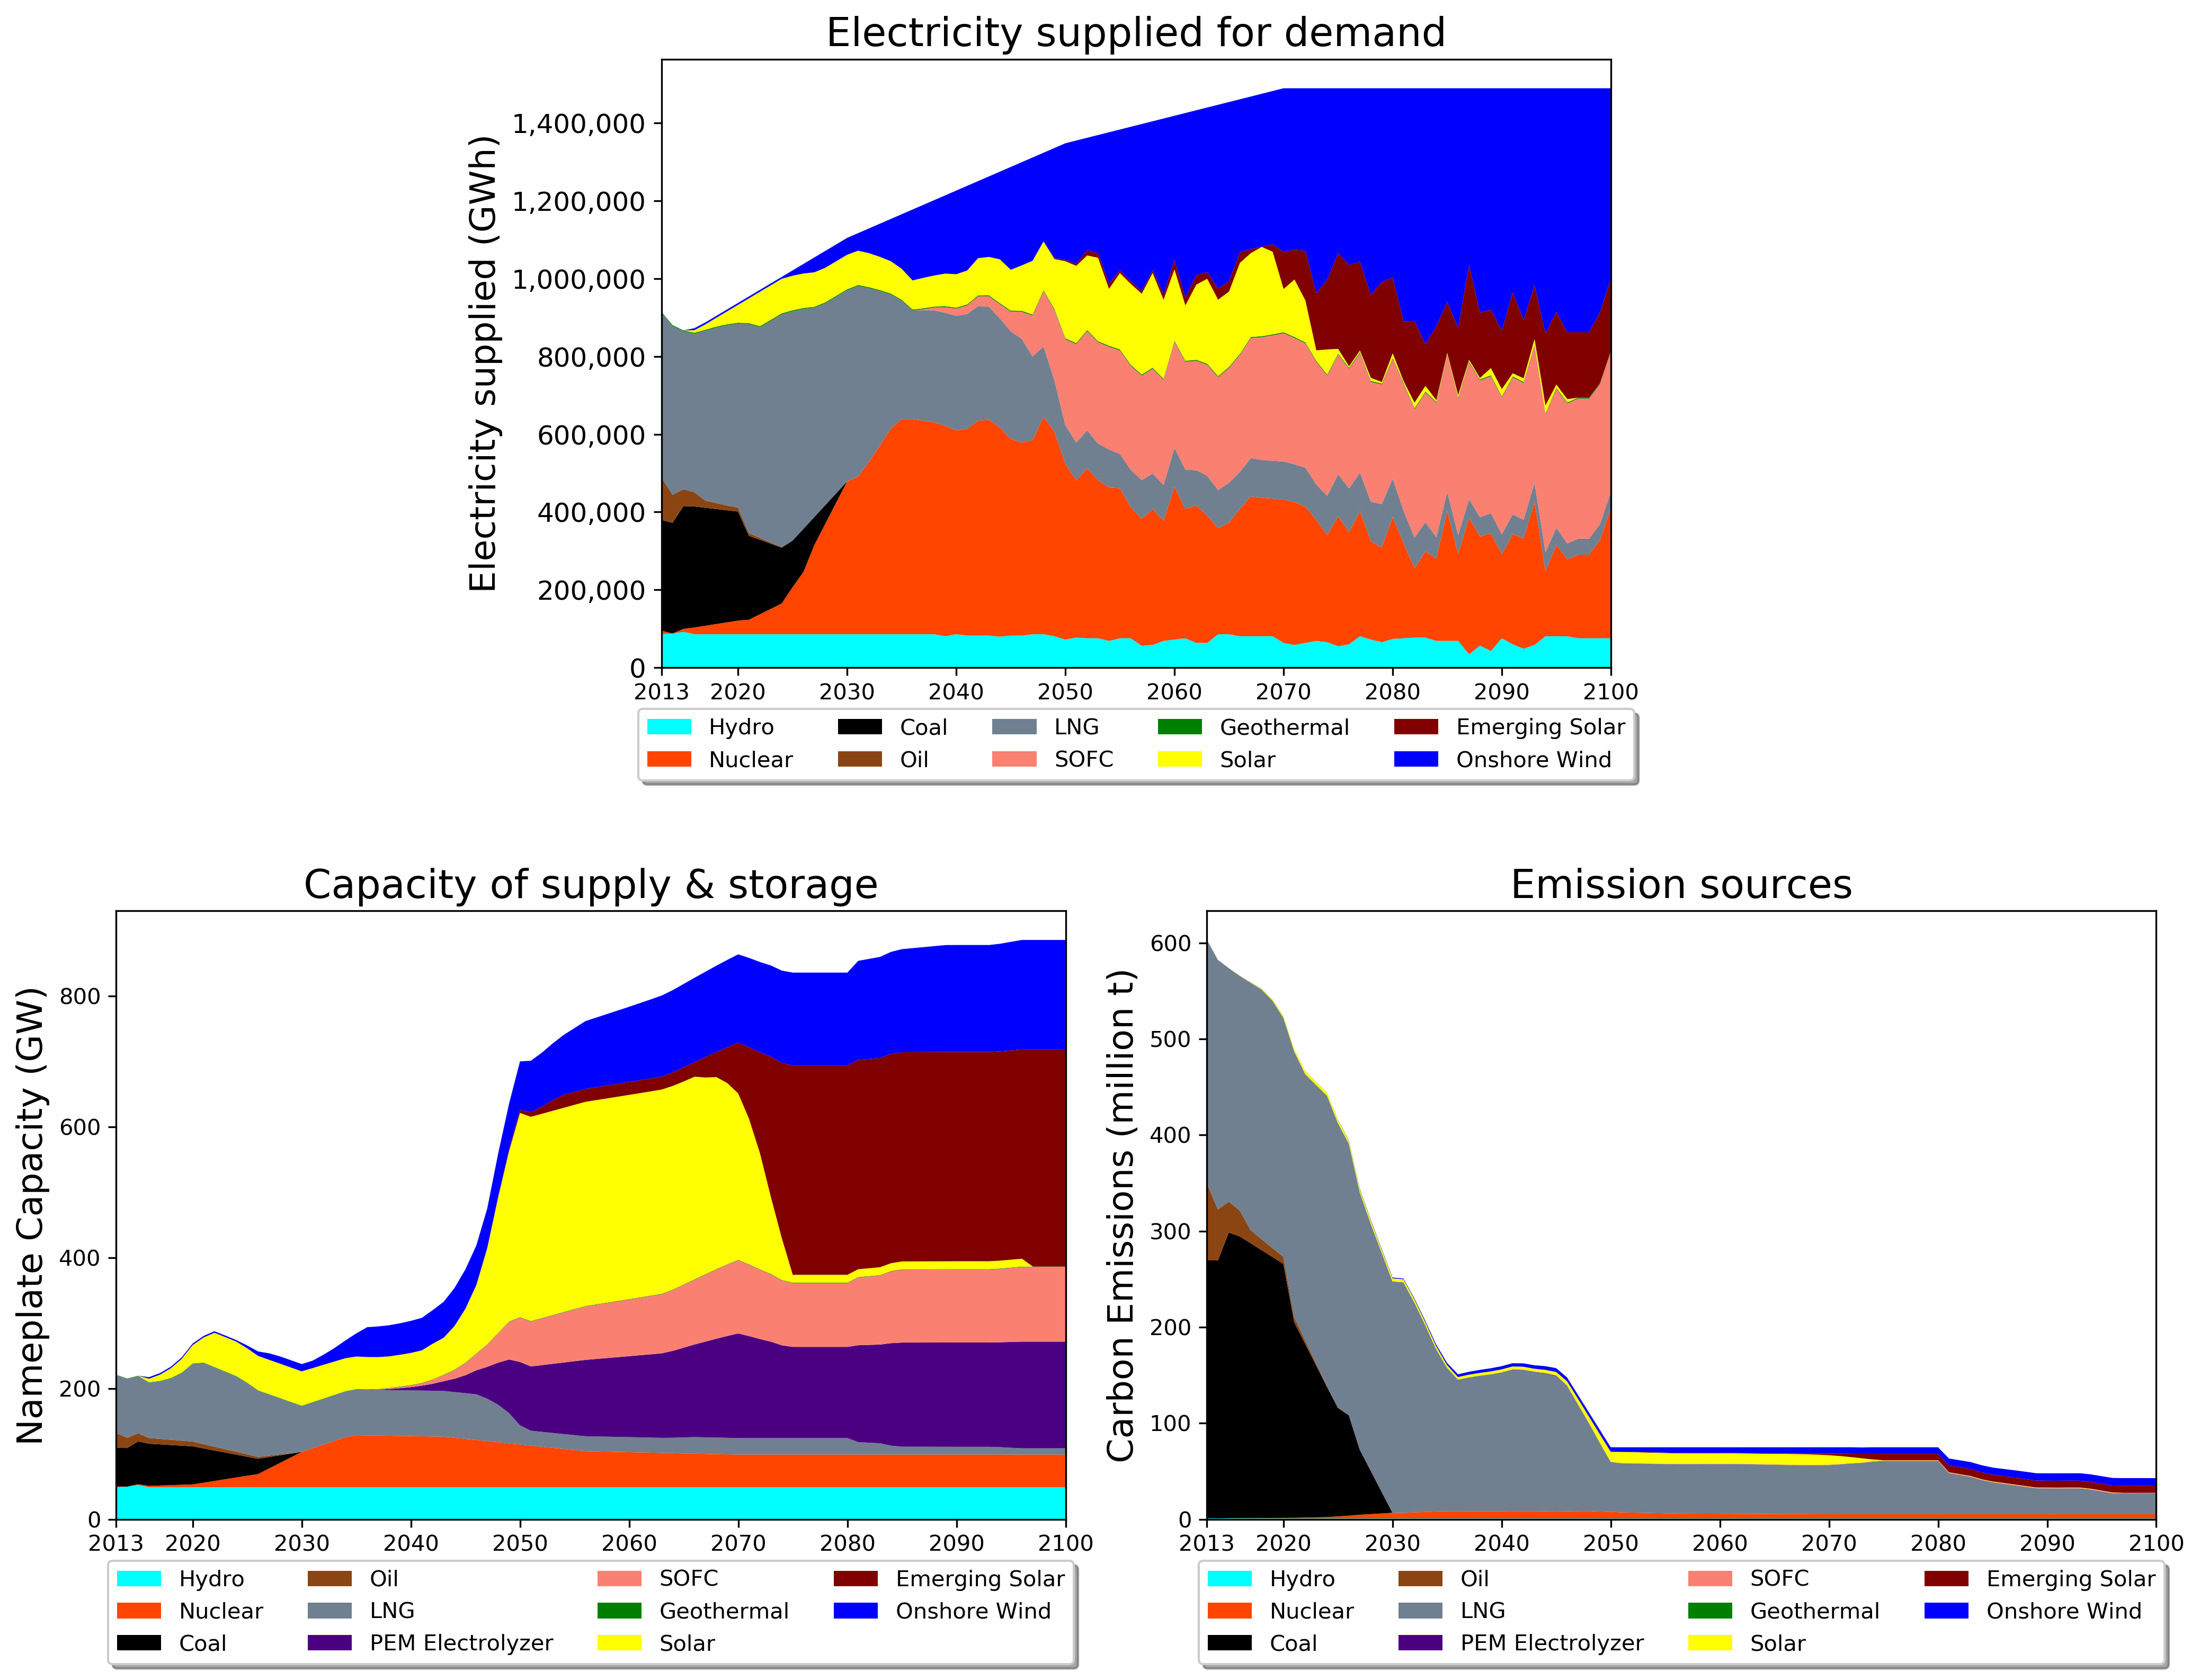
\includegraphics[scale=0.5]{figures/newtechs_nuc}
\caption{Scenario 4 results (emerging technologies with new nuclear). The plot at the top shows the electricity generation mix used to meet the demand, the bottom-left figure shows the nameplate capacities of electricity generation and storage technologies that are deployed to meet the demand, and the bottom-right figure shows the sources of emission(direct and life cycle) resulting from this energy mix.}
\label{scen4}
\end{figure}

The fifth scenario's results (Figure \ref{scen5}) closely resemble those of the third scenario (Figure \ref{scen3}). However, \gls{SOEC}s rapidly replace a large fraction of ageing \gls{PEMEC}s, starting from 2055. Some \gls{PEMEC}s remain in the mix until 2100 despite their lower efficiency due to their lower cost. Both 2030 and 2050 emission targets are met, but no additional emission reductions occur beyond 2050. The amount of electricity diverted to storage technologies is 41,752 TWh, primarily from solar and emerging solar technologies (48\%), onshore wind (28\%), and fixed-bottom offshore wind (20\%). From this, 35,550 TWh of hydrogen is generated, mostly from \gls{SOEC} (56\%), and \gls{PEMEC} (43\%). \gls{AEC} contributes a mere 0.95\% of the total hydrogen, and \gls{PWS} plays the smallest role at 0.05\%. The cost of this transition is \deleted{\textbf{3.18 trillion USD}} \added{3.18 trillion USD}.

\begin{figure}[H] 
\centering
%\vspace*{-3cm}
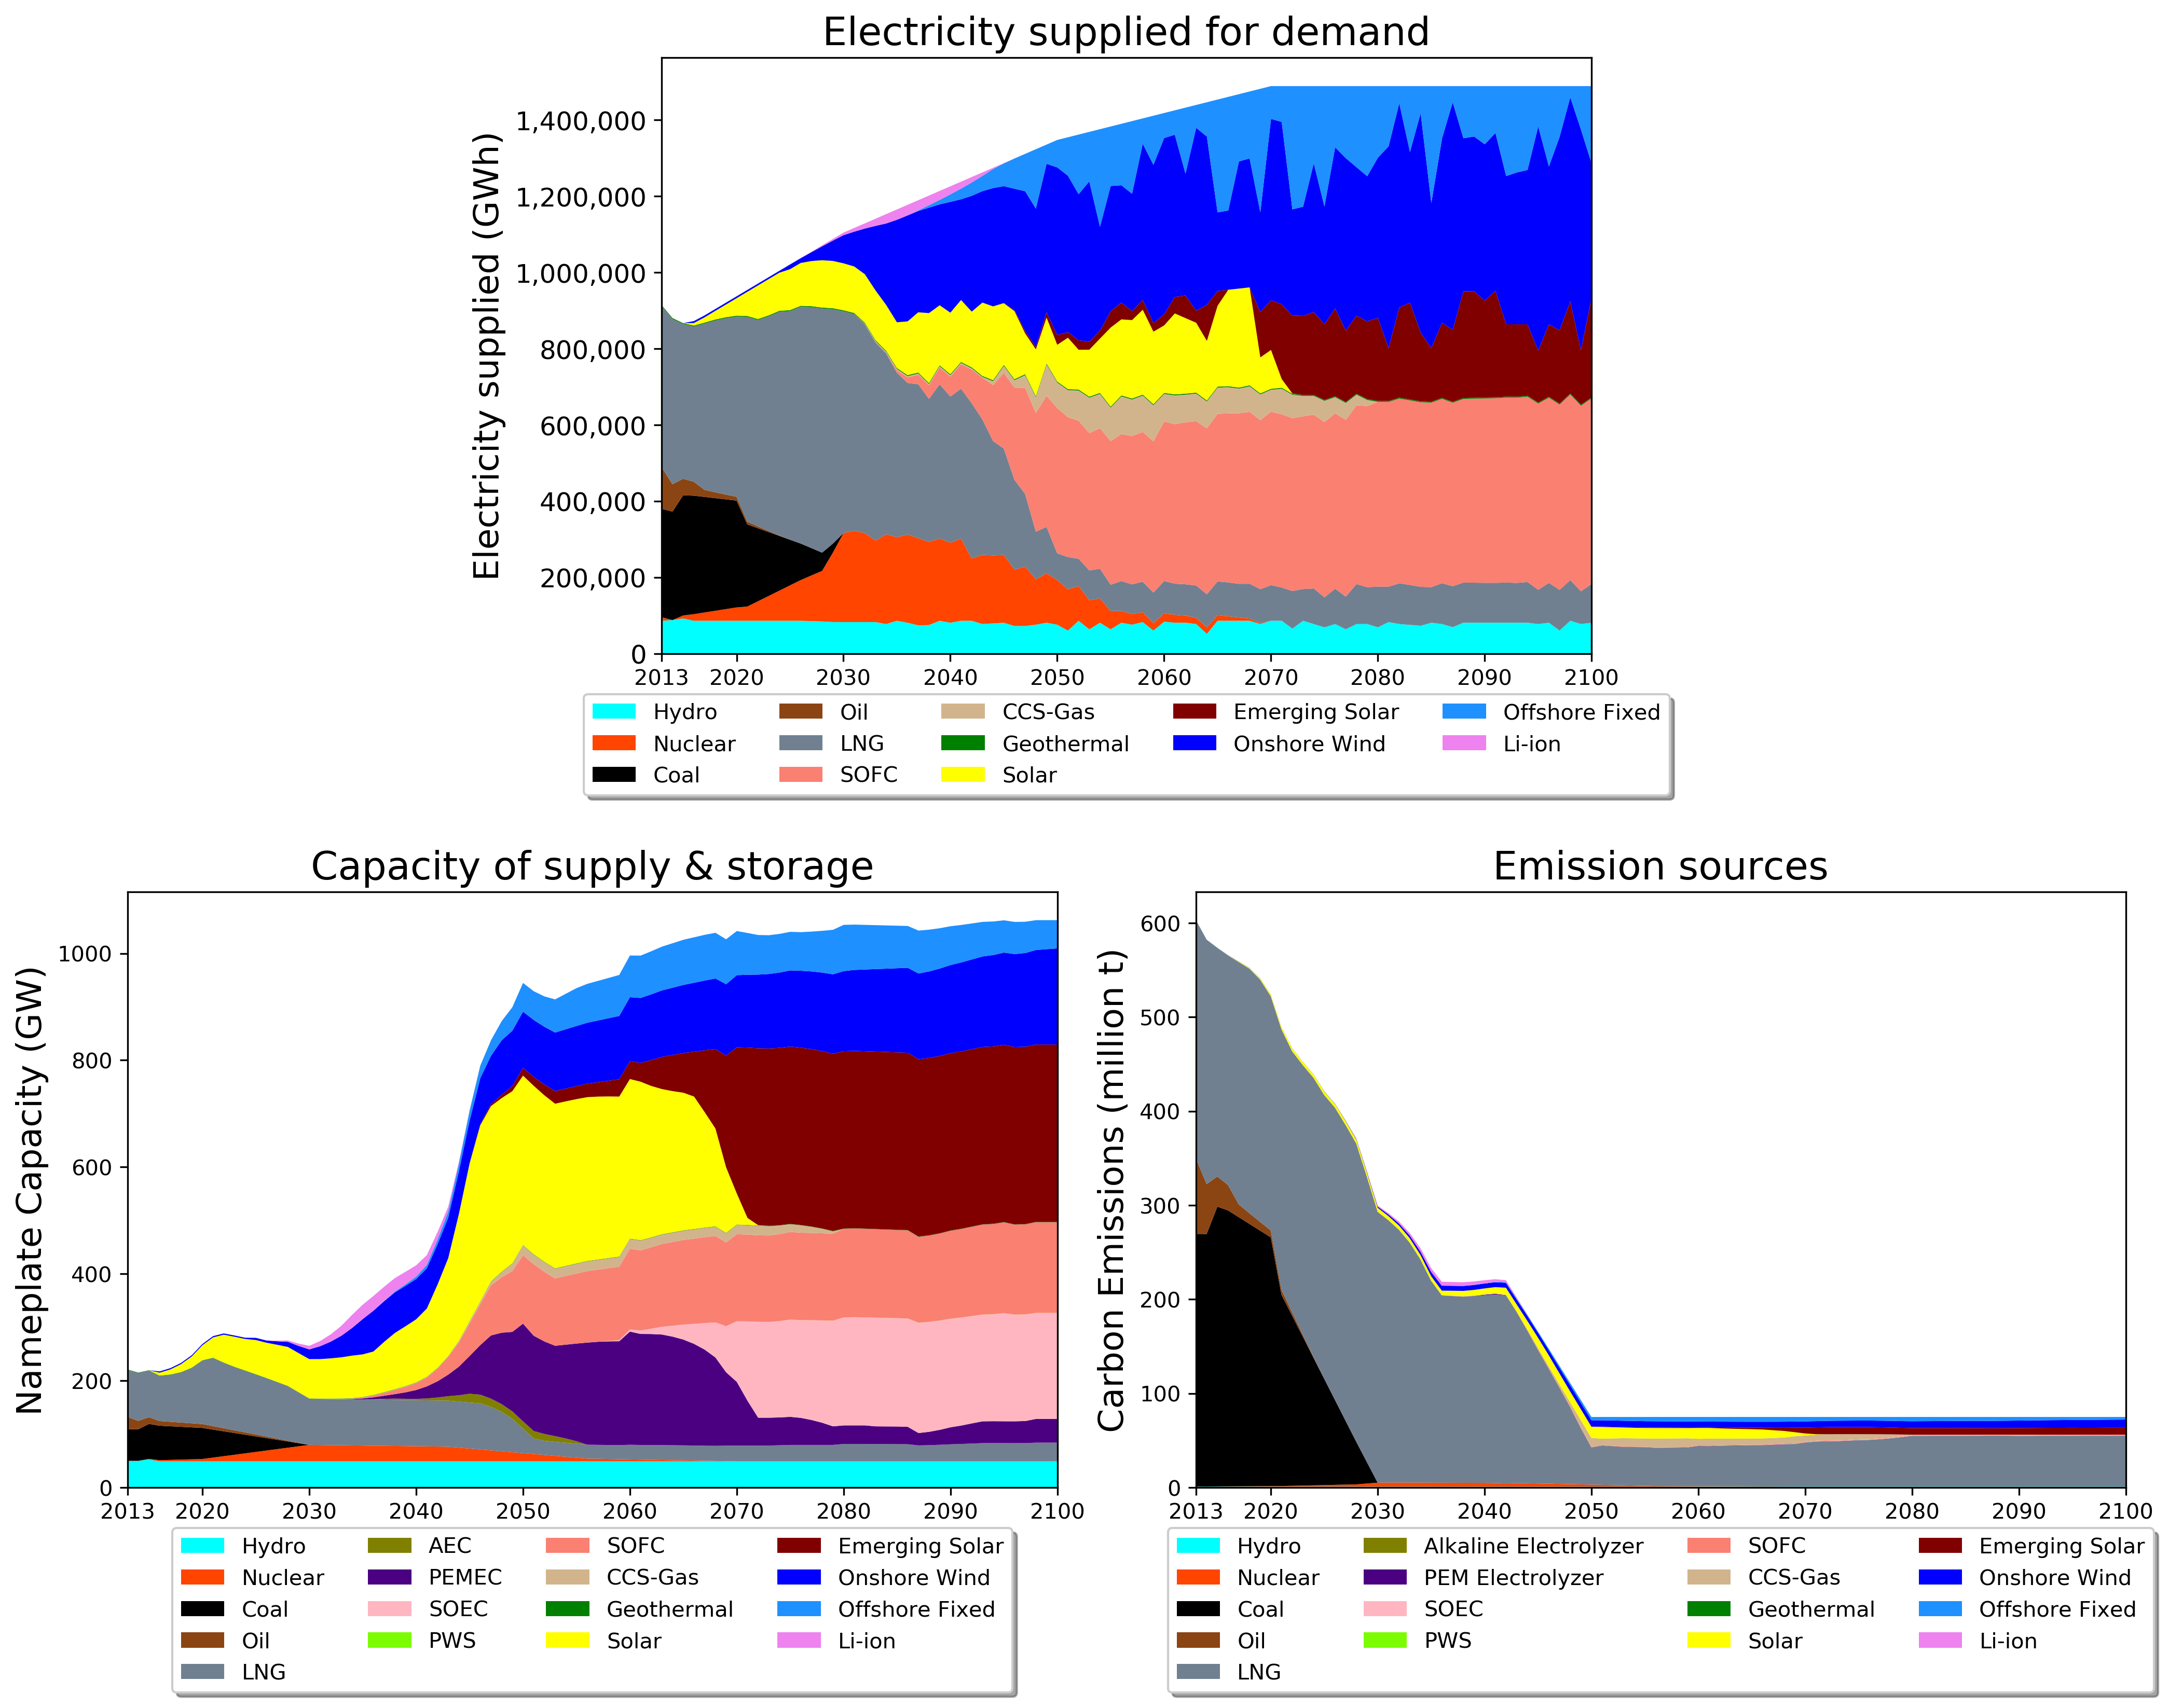
\includegraphics[scale=0.5]{figures/lowtrltech_nonuc}
\caption{Scenario 5 results (emerging technologies and nascent hydrogen technologies without new nuclear). The plot at the top shows the electricity generation mix used to meet the demand, the bottom-left figure shows the nameplate capacities of electricity generation and storage technologies that are deployed to meet the demand, and the bottom-right figure shows the sources of emission(direct and life cycle) resulting from this energy mix.}
\label{scen5}
\end{figure}

\subsection{Sensitivity analysis}

Results from our sensitivity analysis are partially presented in Figures \ref{syscost-smol} and \ref{satechs-smol}, whereas the complete results are in in the appendix (Figs. \ref{pws}-\ref{sa-useless}). The overall transition cost is strongly correlated with the investment cost of \gls{SOFC}s (Figure \ref{satechs-smol}). This follows from the large share of \gls{SOFC}s, as they are the most important low-carbon technology for storing renewable power, yet they are the most expensive technology available to the model. In the absence of new nuclear deployments, \glspl{SOFC} are irreplaceable, and their share is largely fixed. In analysing the sensitivity of the output of electricity generation technologies (Figure \ref{satechs-smol}), we unsurprisingly found the output of \gls{SOFC}s most strongly correlated with their own capital costs. However, the output of \gls{CCS} with natural gas was also most strongly correlated with the investment cost of \gls{SOFC}s, rather than the investment cost of CCS gas itself. The share of \gls{CCS} with natural gas is also relatively small (indicated by the y-values in Figure \ref{satechs-smol}), about 2-3\%.  This is because CCS gas deployment increases only marginally as fuel cells deployment decreases due to increasing fuel cell cost. Therefore, the role of CCS with natural gas is that of a secondary stopgap technology that is deployed when other decarbonisation alternatives are uneconomical. This is due to the large life-cycle and direct emissions of CCS gas compared to renewables and hydrogen technologies.

\begin{figure}[H] 
\centering
\hspace*{-1cm}
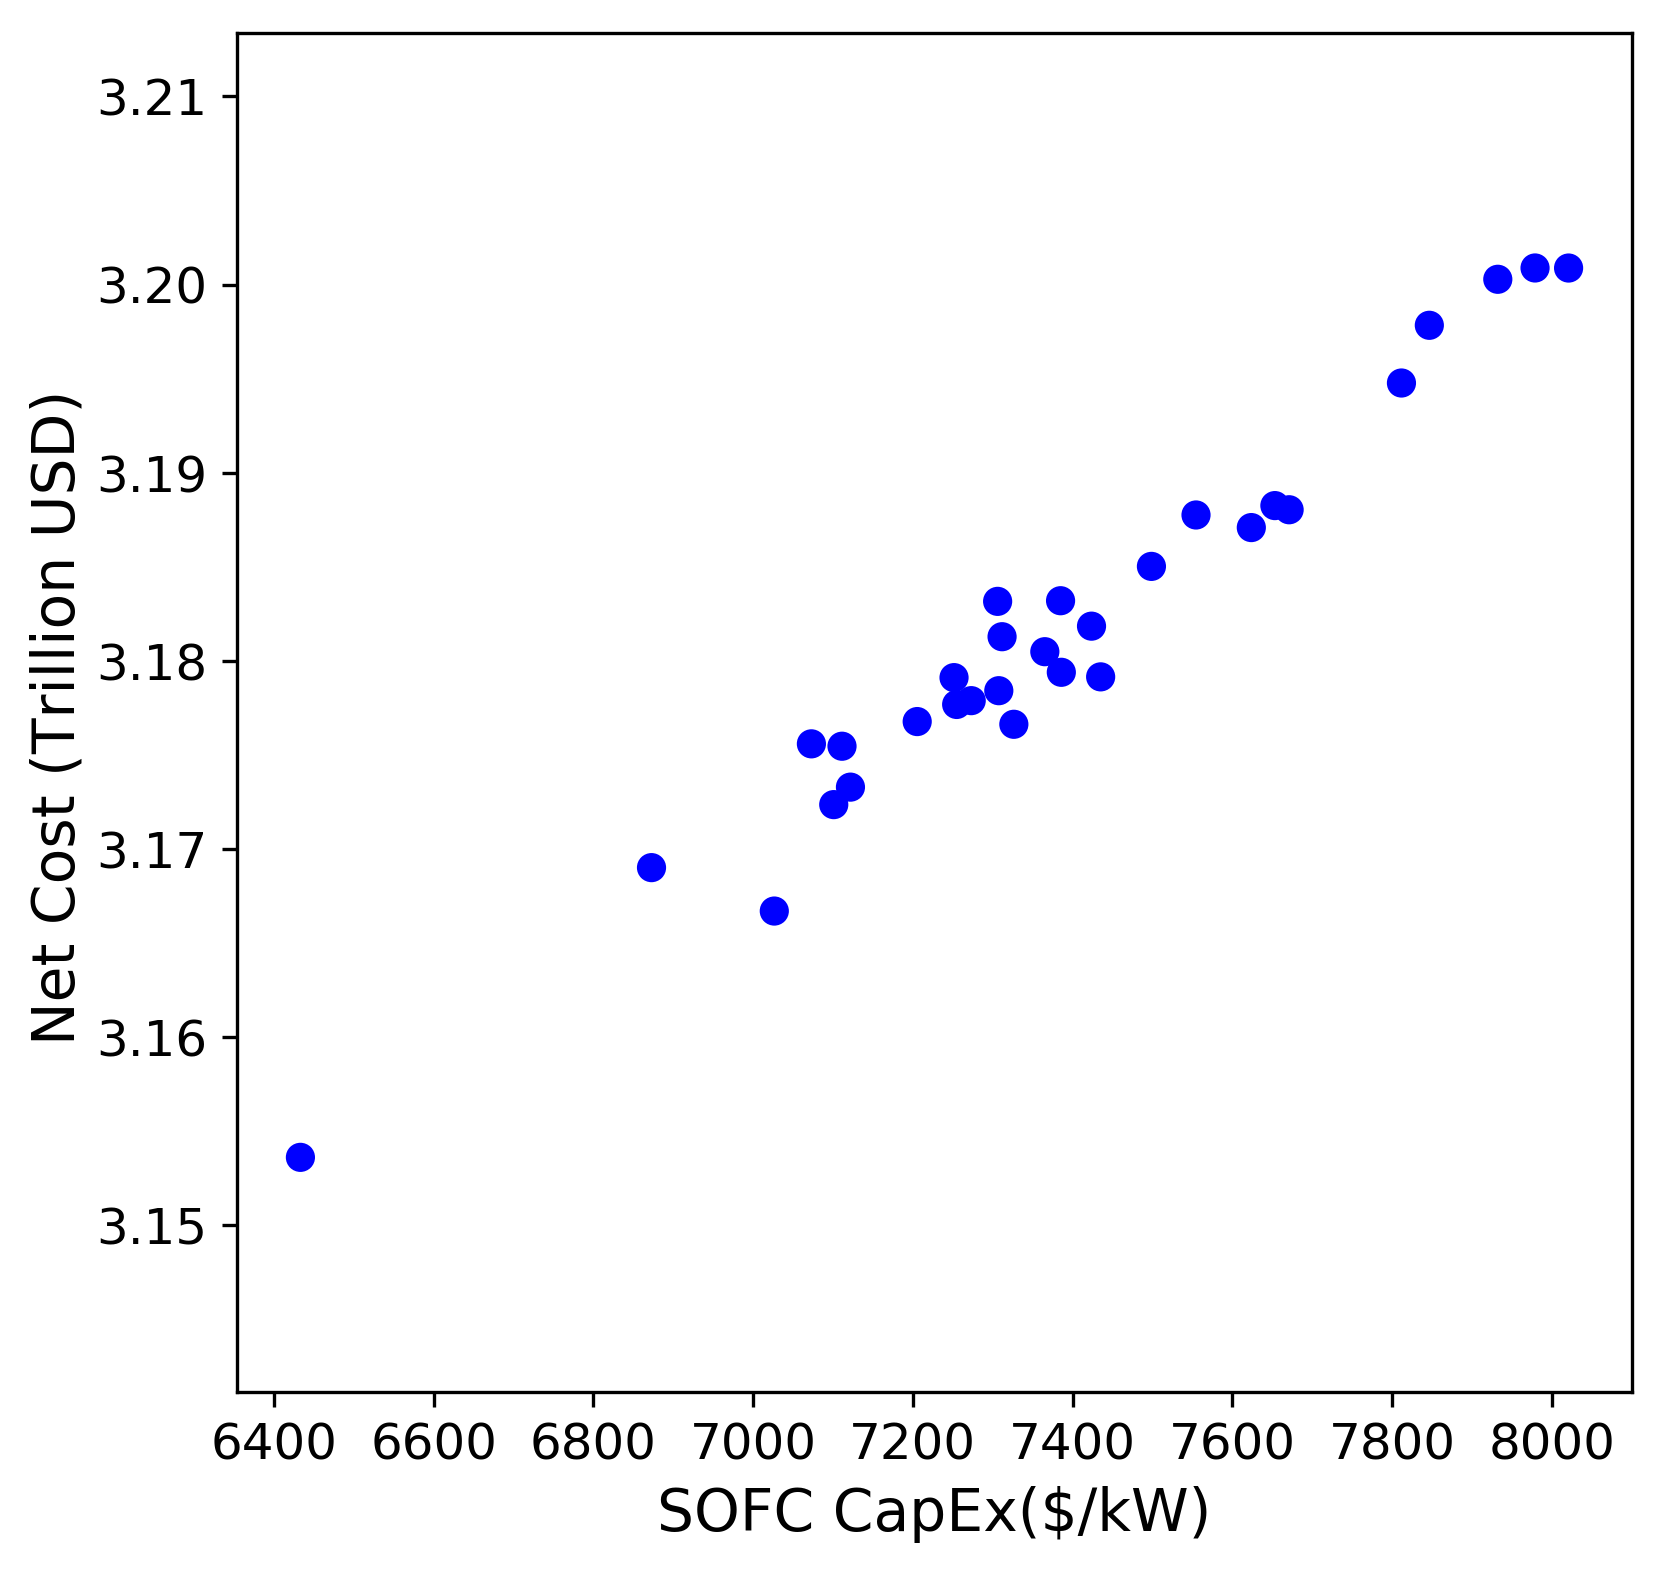
\includegraphics[scale=0.7]{figures/syscost_abbrv}
\caption{Sensitivity analysis for overall transition cost vs. solid oxide fuel cell capital costs.}
\label{syscost-smol}
\end{figure}

\begin{figure}[H] 
\centering
%\hspace*{-3cm}
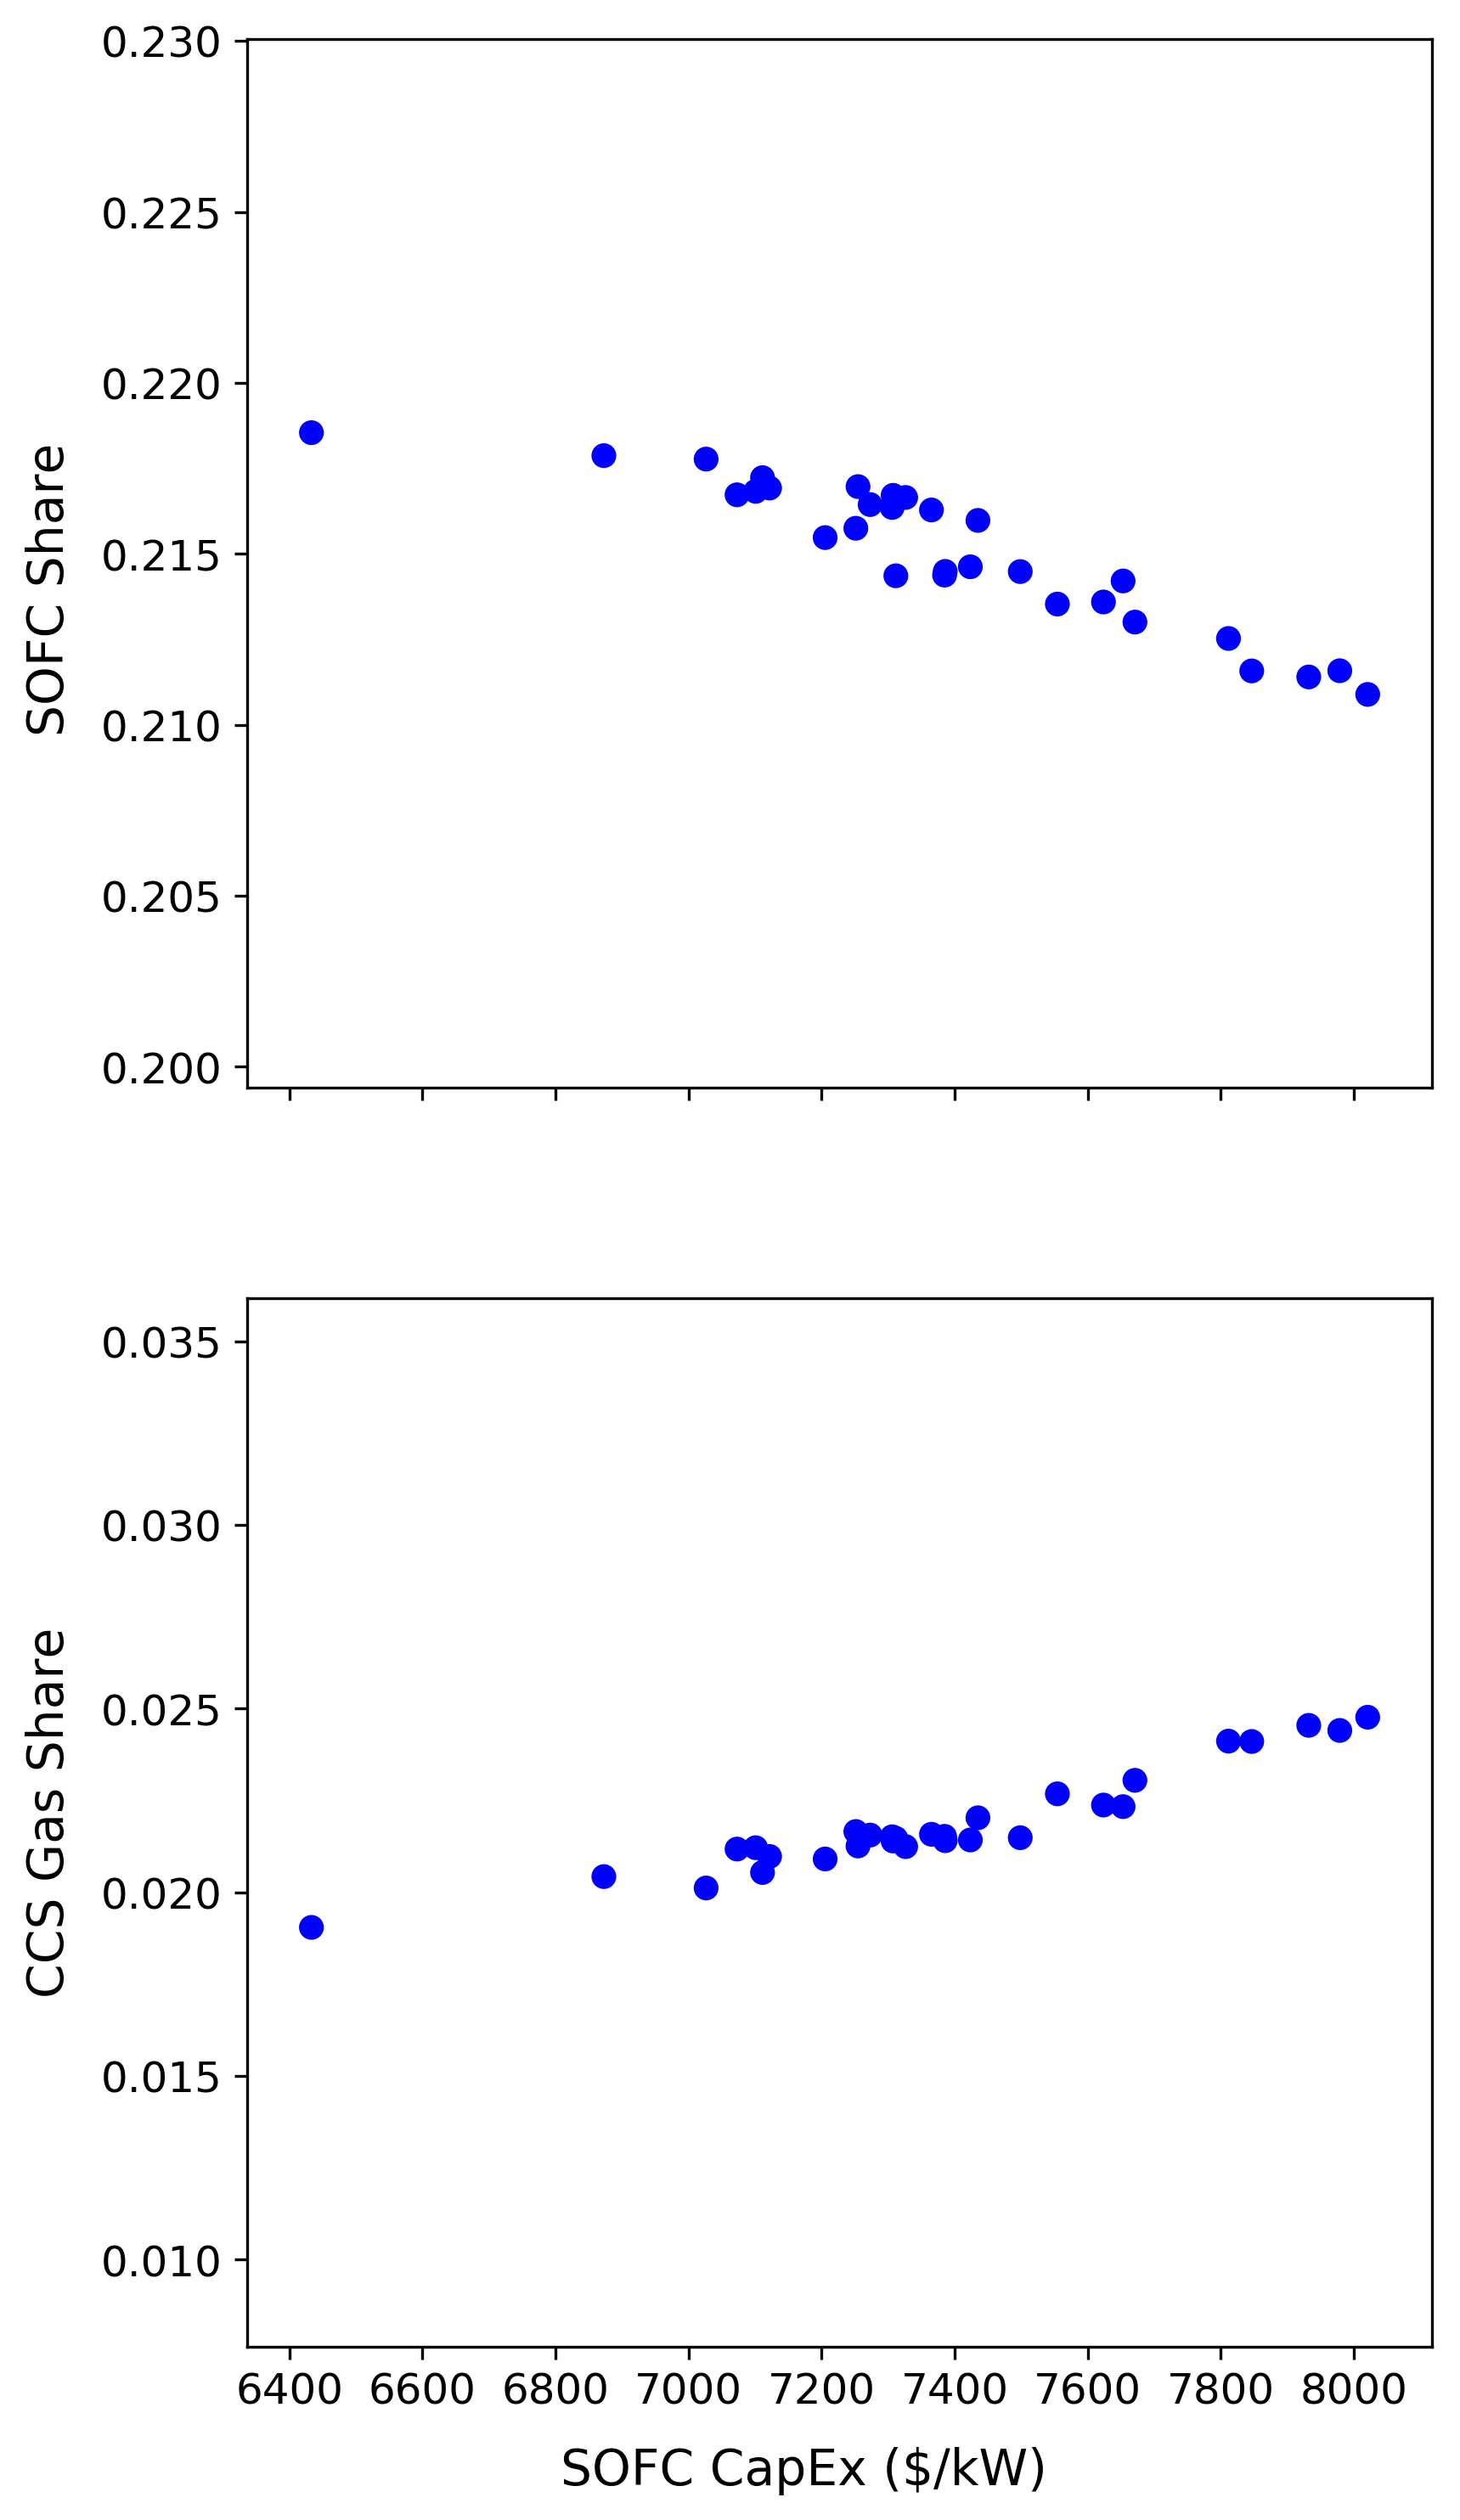
\includegraphics[scale=0.7]{figures/satechselc_abbrv}
\caption{Sensitivity analysis results for electricity supply shares of solid oxide fuel cells (top) and carbon capture and sequestration natural gas plants (bottom) vs solid oxide fuel cell capital costs.}
\label{satechs-smol}
\end{figure}

Remaining results indicate that \gls{PEMFC}s are never utilised because of their low efficiency compared to \gls{SOFC}s, and \gls{CCS} coal plants are never deployed due to their high emission coefficient (Figure \ref{sa-useless}). \gls{PWS} plays a minor role in generating 0-20 TWh of hydrogen over the entire simulation's time-period (Figure \ref{pws}), as opposed to \gls{SOEC}s which generate 19,500-22,500 TWh, and \gls{PEMEC}s, which generate 12,000-16,000 TWh of hydrogen, respectively. The share of \gls{PWS} was found to be strongly correlated with its investment cost, with \$3300/kW the approximate threshold at which this technology ceases to be cost-competitive (Figure \ref{pws}). \gls{PWS} deployment is also weakly correlated with the splitting efficiency; values over 21\% seem most favourable. The \gls{PWS} emission coefficient is too small to have an impact on the overall emissions of the system considering \gls{PWS}'s small deployment. Hence its emission coefficient does not appreciably affect \gls{PWS} deployment. Since \gls{PEMFC}s, \gls{CCS} coal, and \gls{PWS} are not deployed in quantities significant enough to affect the model's performance, they are omitted as potential dependent variables for the rest of the sensitivity analysis.

For hydrogen generating technologies (Figure \ref{satechs-h2}), the \gls{SOEC} output is most strongly correlated with the SOEC investment cost. However, \gls{SOEC} output is affected insignificantly by the perturbation applied to its investment cost. \gls{SOEC} deployment is largely insensitive to its emission coefficient as its contribution to overall emissions is negligible. This highlights \gls{SOEC}'s vital role in the transition. \gls{PEMEC} (Figure \ref{satechs-elc}) deployment is also most noticeably affected by its respective investment costs, but also by the investment cost of SOECs - as SOECs become more expensive, \gls{PEMEC}s emerge as the natural replacement.
\FloatBarrier
\section{Discussion}
% This should explore the significance of the results of the work, not repeat
% them. A combined Results and Discussion section is often appropriate. Avoid
% extensive citations and discussion of published literature.

%Notes for Ansh:
%Importance of nuclear : cost of various transitions, flexibility by itself and when coupled with storage (Li-ion, H2). How it precludes the need for CCS.
%Urgency of transition : scenarios + sensitivity analysis.
%Li-ion storage: land use requirements for each case, qualitatively discuss Co, Ni requirements. Say Li is okay.
%AECs,PEMECs,SOECs need to be highly flexible with high availability factors.
%SOFCs: need for extremely responsive SOFCs with high availability factor, flexible operation (cite challenges from NREL).
%pemecs still part of cost optimal solutions
%identify key techs, same fcs needed always
%nuclear is key
%pws will have to be cheaper/cost competitive with electrolyzers to have a role
%main H2, role of CCS LNG - secondary alternative to H2 - as shown by correlation with SOFC inv cost. Not good on its own. Supplement to H2.
%H2 non trivial despite large range of perturbation
% FC flexibility, more storage/H2 less flex for CCS, nuclear

%urgency
As the results of all base case scenarios indicate, rapid retirement of fossil fuels and deployment of carbon neutral technologies is urgently required to achieve emission reduction targets in Japan. All coal and oil plants need to be shut down between 2025-2030, and natural gas use must be reduced dramatically. It is also imperative that the existing nuclear reactors be operated at full capacity by 2022. Since hydrogen plays a key role in zero to moderate nuclear deployment scenarios (Figs. \ref{scen3} and \ref{scen4}), it appears prudent to invest in hydrogen power. As the model uses learning curves for technology prices, and our objective function is transition cost, hydrogen technologies are deployed as late as possible to minimise costs by utilising technologies at their cheapest, while there is still time to deploy them and achieve emission goals. Therefore, results indicate that it is imperative that Japan deploy an increasing amount of renewables, including wind power, between 2020-2030, and be prepared to deploy and rapidly scale up hydrogen power by 2030 at the latest in the absence of new nuclear, or by 2035 with new nuclear.

%nuclear
The scenario with the maximum nuclear deployment, Scenario 2, also has the lowest transition cost. When used with hydrogen, 50 MW of new nuclear results in the greatest reduction in emissions after 2050 out of all 5 scenarios. It also reduces the cost of the transition from 3.18 trillion USD in Scenario 3 to 2.80 trillion USD in Scenario 4, a difference of 12\% of the system cost. The estimated savings in cost and emissions due to nuclear are conservative, as we have not incorporated the cost of transporting hydrogen utilising tankers or pipelines. The large emission cuts achieved with the help of nuclear also allow natural gas to continue operating until 2100 while meeting emission goals. As natural gas is well suited to peaking and load-following, when coupled with flexible fuel cell technologies, it could engender in an extremely stable energy system. 

For the transitioning energy system in Japan, under all scenarios investigated, nuclear plays a key role in reducing emissions. A potential strategy for Japan could include the reinvigoration of its nuclear energy sector by restarting existing plants and, if politically feasible, constructing new plants and investing in advanced reactor research. To minimise the environmental impact from life cycle emissions, it is necessary that all existing and any new reactors be operated for a lifetime of 60 years or more at a high capacity factor. Premature decommissioning due to operational problems or lack of public acceptance need to be avoided. Therefore, prioritising reactor safety for resilience to disasters and in order to regain the public's trust in nuclear power, and increasing public awareness of nuclear's vital role in mitigating carbon emission are key to achieving 2030 and 2050 emission targets.

%renewables and flexibility
In all scenarios, solar and wind supply a large portion of the electricity demand. Unless large numbers of nuclear power plants are constructed, Japan will need to invest heavily in offshore wind farms by 2030 (Figs. \ref{scen1}, \ref{scen3}-\ref{scen5}). If hydrogen and CCS are not deployed by 2035, investment in offshore floating turbines may also become necessary (Fig. \ref{scen1}). In a scenario with a relatively large share of renewables, grid flexibility becomes extremely important. Such a scenario requires significant investment in storage technologies and ensuring that all emerging technologies are flexible and responsive. As natural gas is the only extant option for prompt load-following, it is necessary to invest in nuclear or hydrogen to achieve emission cuts while simultaneously keeping natural gas operational. Additionally, any nuclear power plants and fossil fuel power plants which use CCS must be able to load-follow or be coupled to storage, ideally electrolysers, in order to store excess electricity for peak demand, and potentially utilise waste heat for hydrogen generation. Any fuel cell technology utilised must also be extremely flexible and responsive. Since the model prioritises \gls{SOFC}s over \gls{PEMFC}s due to their higher efficiency, it is important that \gls{SOFC}s reduce their startup times to have an edge over \gls{PEMFC}s in utility-scale applications.

%batteries
Lithium-ion batteries are the preferred storage medium in the absence of hydrogen. However, as the base case scenarios indicate, extremely large capacities of storage must be deployed to achieve a stable grid that can sustain the large capacities of renewables required for deep emission cuts. While lithium may be available, cobalt and manganese reserves are limited \cite{scrosati_lithium-ion_2011,simon_potential_2015,turcheniuk_ten_2018} , which may inflate the prices of lithium-ion storage if it is relied upon as the primary storage medium. It may be preferable to redesign batteries to reduce the amount of rare minerals used in their manufacturing and improve recycling to increase the recovery rate of rare metals. The life cycle emissions from batteries must also be reduced by using cleaner materials and electricity for manufacturing. If hydrogen storage is available, battery storage serves as a near-term transition technology after which hydrogen storage dominates (Figs. \ref{scen3}-\ref{scen5}).

%hydrogen - key players, key parameters, path forward?
After nuclear, hydrogen power emerges as the second most effective technology for achieving 2050 emission goals. As seen in the sensitivity analysis results, hydrogen maintains a significant share of the electricity mix despite a wide range of perturbations to key parameters of the hydrogen sector. While \gls{SOFC}s and \gls{SOEC}s are preferred over \gls{PEMFC}s and \gls{PEMEC}s in all of our simulations, the role of hydrogen is so important that if \gls{SOFC} or \gls{SOEC} deployment is disabled, the model replaces them with inferior \gls{PEMFC}s or \gls{PEMEC}s, respectively, to recreate similar energy mixes. Key technologies that aid in decarbonisation in our simulations are \gls{SOFC}s and \gls{PEMEC}s. Steam reforming, with or without CCS, does not get utilised in our simulations due to its high emission coefficient. At the lower end of the technology readiness scale, \gls{SOEC}s emerge as tremendously disruptive due to their high efficiency. However, their operational lifetimes need to be increased significantly, life cycle emissions must be kept low, and cost-competitiveness with \gls{PEMEC}s must be achieved in order to realise their potential. \gls{PWS} plays a marginal role as it is not cost-competitive with electrolysis. From the sensitivity analysis results, the investment cost of \gls{SOFC}s emerges as a critical parameter. Therefore it is vital to reduce fuel cell investment costs to make deep emission reduction economically feasible. Low response times and high availability of fuel cells and electrolysers are two other desirable traits that are implicit in our assumptions. If \gls{SOFC}s are not as flexible as assumed, they are replaced in our simulations by \gls{PEMFC}s, which are known to be more flexible. Hence, our results show that the more flexible and responsive hydrogen technologies will be dominant in a renewable energy-based transition. In Scenarios 3 and 4, solar, wind, and nuclear are used to generate hydrogen. It would be economically favourable to couple utility-scale renewables and nuclear power plants with electrolysis plants. The use of waste heat from nuclear to produce hydrogen would reduce reliance on renewables for electrolysis, and mitigate intermittency-related grid-stability issues.

%ccs
CCS plays a small role in our base case scenarios as a transitional technology. Despite being cheaper than hydrogen, its share is found to be largely insensitive to its investment costs as evidenced by the sensitivity analysis. This is mainly due to the large emission coefficient of \gls{CCS} with natural gas. Marginal gains are expected in \gls{CCS} penetration if the capture efficiency is increased to reduce its direct emissions. Reducing indirect emissions is likely to have a greater impact on \gls{CCS} penetration. This could be achieved by increased electrification of the industrial sector and the use of hydrogen to produce steel.

Our policy-agnostic analysis relies on optimal solutions and scenarios. However, policy makers in Japan are considering two alternatives as to the long-term nature of the low-carbon energy system. One approach could prioritise nuclear energy and reap the benefits of inexpensive, low-carbon energy if consensus from the public for its long-term deployment and use can be achieved. Another low carbon energy pathway proposed by our results is a transition toward a hydrogen economy, utilising hydrogen as a storage medium to engender significant deployment of renewable energy. The hydrogen pathway also provides more energy security. As social opposition to nuclear power is a prominent issue in Japan, the deployment of a parallel nuclear and hydrogen-based energy system is unlikely. Nonetheless, our results indicate that these two approaches are not mutually exclusive. The cost of transitioning to a hydrogen energy system without deploying any new nuclear is much higher than that of any of the nuclear-inclusive options. Deploying nuclear in tandem with hydrogen provides a cost-effective compromise. An approach reliant on a mature technology like nuclear also improves the likelihood of Japan meeting its 2050 emission goals, as the timely success of the Japanese hydrogen plan is far from certain \added{especially considering the more ambitious carbon reduction goals recently announced by METI \mbox{\cite{noauthor_japans_2021,yamaguchi_japan_2021}}} . At the very least, as is the case for CCS and fossil fuels, nuclear power may offer a ``bridging" option, providing a low-carbon pathway in the short-term through extended nuclear lifetimes and limited new builds, allowing sufficient time for the maturation of hydrogen and renewable-based energy options for long-term deployment. If supported politically, long-term use of nuclear power could provide emission cuts well beyond the 2050 targets. Policy which is cognizant of these economic, environmental, and social aspects of energy systems is required to deliver a low-cost, low-carbon energy future for Japan which is socially acceptable.
\FloatBarrier
\section{Conclusion} \label{Conclusion}
%what we did. sum up key technologies, what needs to happen for technologies that are not "key", importance of rapid change/suggested timeline.

We simulated five transition scenarios which assess potential pathways to meeting 2030 and 2050 emission targets within the Japanese electricity supply system and their long-term impact up to 2100. Scenario 1 (Figure \ref{scen1}) proved that meeting emission goals without new nuclear or new low-emission technologies is infeasible, and such an endeavour is likely to be an expensive failure. The remaining scenarios demonstrate that emission goals can be met by either investing heavily in nuclear (Figure \ref{scen2}), investing heavily in hydrogen (Figs. \ref{scen3} and \ref{scen5}), or using a combination of both (Figure \ref{scen4}). Scenarios that incorporate nuclear are the most cost-effective, and using a combination of nuclear and hydrogen leads to the greatest emission reduction post-2050. Key technologies that emerge from are results include nuclear power and hydrogen from renewables, while \gls{CCS} with natural gas and photochemical water splitting (\gls{PWS}) play a nominal role. CCS with coal, steam reforming with or without CCS, new coal, and new oil are not utilised due to their high direct and life-cycle emissions. Our analysis indicates that while politically challenging, a hybrid nuclear-hydrogen strategy is economically feasible and results in long-term emission reduction. Such a multifaceted approach to emission reduction is also likely to improve decarbonisation outcomes since the commercialisation and deployment of hydrogen in time to meet 2030 and 2050 emission goals is uncertain.

Mitigating emissions from the industrial and transportation sector presents unique challenges that may affect the amount of emission reduction required from the electricity supply sector to meet Japan's 2030 and 2050 goals. Future work should incorporate holistic assessment of the entire Japanese energy system when exploring energy transition pathways. The assessment of synergistic utilisation of hydrogen in transportation and industry alongside electricity storage and supply is vital for policy decisions. The effect of transportation media such as trucks and pipelines on hydrogen and CCS is also worth investigating. \added{Any new technologies that develop in the future and promise rapid decarbonisation should also be incorporated in such work.} Finally, economic feasibility analyses with respect to national budget requirements and projected GDP trends must also be conducted to improve decarbonisation strategies, improve social outcomes, and delineate investment goals for the energy sector.

%\section{Future work}
%grid resilience - analysis of grid stability of similar mixes at the resolution of minutes. Maybe in TIMES (ugh).
%\section{Declaration of Competing Interest}
%The authors declare no conflict of interest.
\FloatBarrier
\section{Acknowledgments}

The author(s) gratefully acknowledge the support of the International Institute for Carbon Neutral Energy Research (WPI-I2CNER), sponsored by the Japanese Ministry of Education, Culture, Sports, Science and Technology. We are also grateful to Kenshi Itaoka and Hadi Farabi-Asl for providing valuable discussions related to this project, and to Gavin Davis and Nataly Panczyk for editing drafts.

The authors contributed to this work as described below.

Anshuman Chaube designed simulation models, conducted sensitivity analysis, and wrote the original draft of the paper.

Andrew Chapman conceived and contributed to conception of the simulations, designed simulation models, and wrote the original draft of the paper. 

Akari Minami translated data from Japanese to English, and assisted with testing and performing simulations.

James Stubbins supervised the work, conceived and contributed to conception of the simulations, and reviewed drafts of the paper.

Kathryn D. Huff supervised the work, conceived and contributed to conception of the simulations, and reviewed drafts of the paper.  Prof. Huff is supported by the Nuclear Regulatory Commission Faculty Development Program, the National Center for Supercomputing Applications, the International Institute for Carbon Neutral Energy Research (WPI-I2CNER), sponsored by the Japanese Ministry of Education, Culture, Sports, Science and Technology, and  DOE ARPA-E MEITNER program award DE-AR0000983.

\FloatBarrier
\bibliographystyle{elsarticle-num}
\bibliography{i2cner-paper-2}
\newpage
\appendix
\section{Model data and assumptions} \label{Appendix}

\begin{table}[H]
\centering
	\caption{Data for defining the initial condition across all simulations.}
	\vspace{0.1in}
	\begin{tabularx}{0.75\textwidth}{p{0.15\textwidth} p{0.15\textwidth} p{0.2\textwidth} p{0.25\textwidth}}
		\hline
\textbf{Technology} & \textbf{\gls{lcoe}} \cite{lazard_lazards_2016} & \textbf{Emission} & \textbf{Year of total}\\
  & (USD/kWh) & \textbf{coefficients} \cite{noauthor_electricity_2019} (gCO$_2$-eq. /kWh) & \textbf{retirement} \\
\hline
Coal & 0.06 & 943 & 2030 \\
\gls{lng} & 0.08 & 599 & 2030 \\
Oil & 0.39 & 738 & 2030 \\
Nuclear & 0.11 & 21 & 2069 \\
Hydro & 0.05 & 11 & N.A. \\
Geothermal & 0.12 & 13 & N.A. \\
Wind & 0.11 & 25 & 2040 \\
Solar & 0.15 & 37 & 2040 \\
\hline 
\end{tabularx}
\label{init-eco}
\end{table}

\begin{figure}[h] 
\centering
\label{ic-elc}
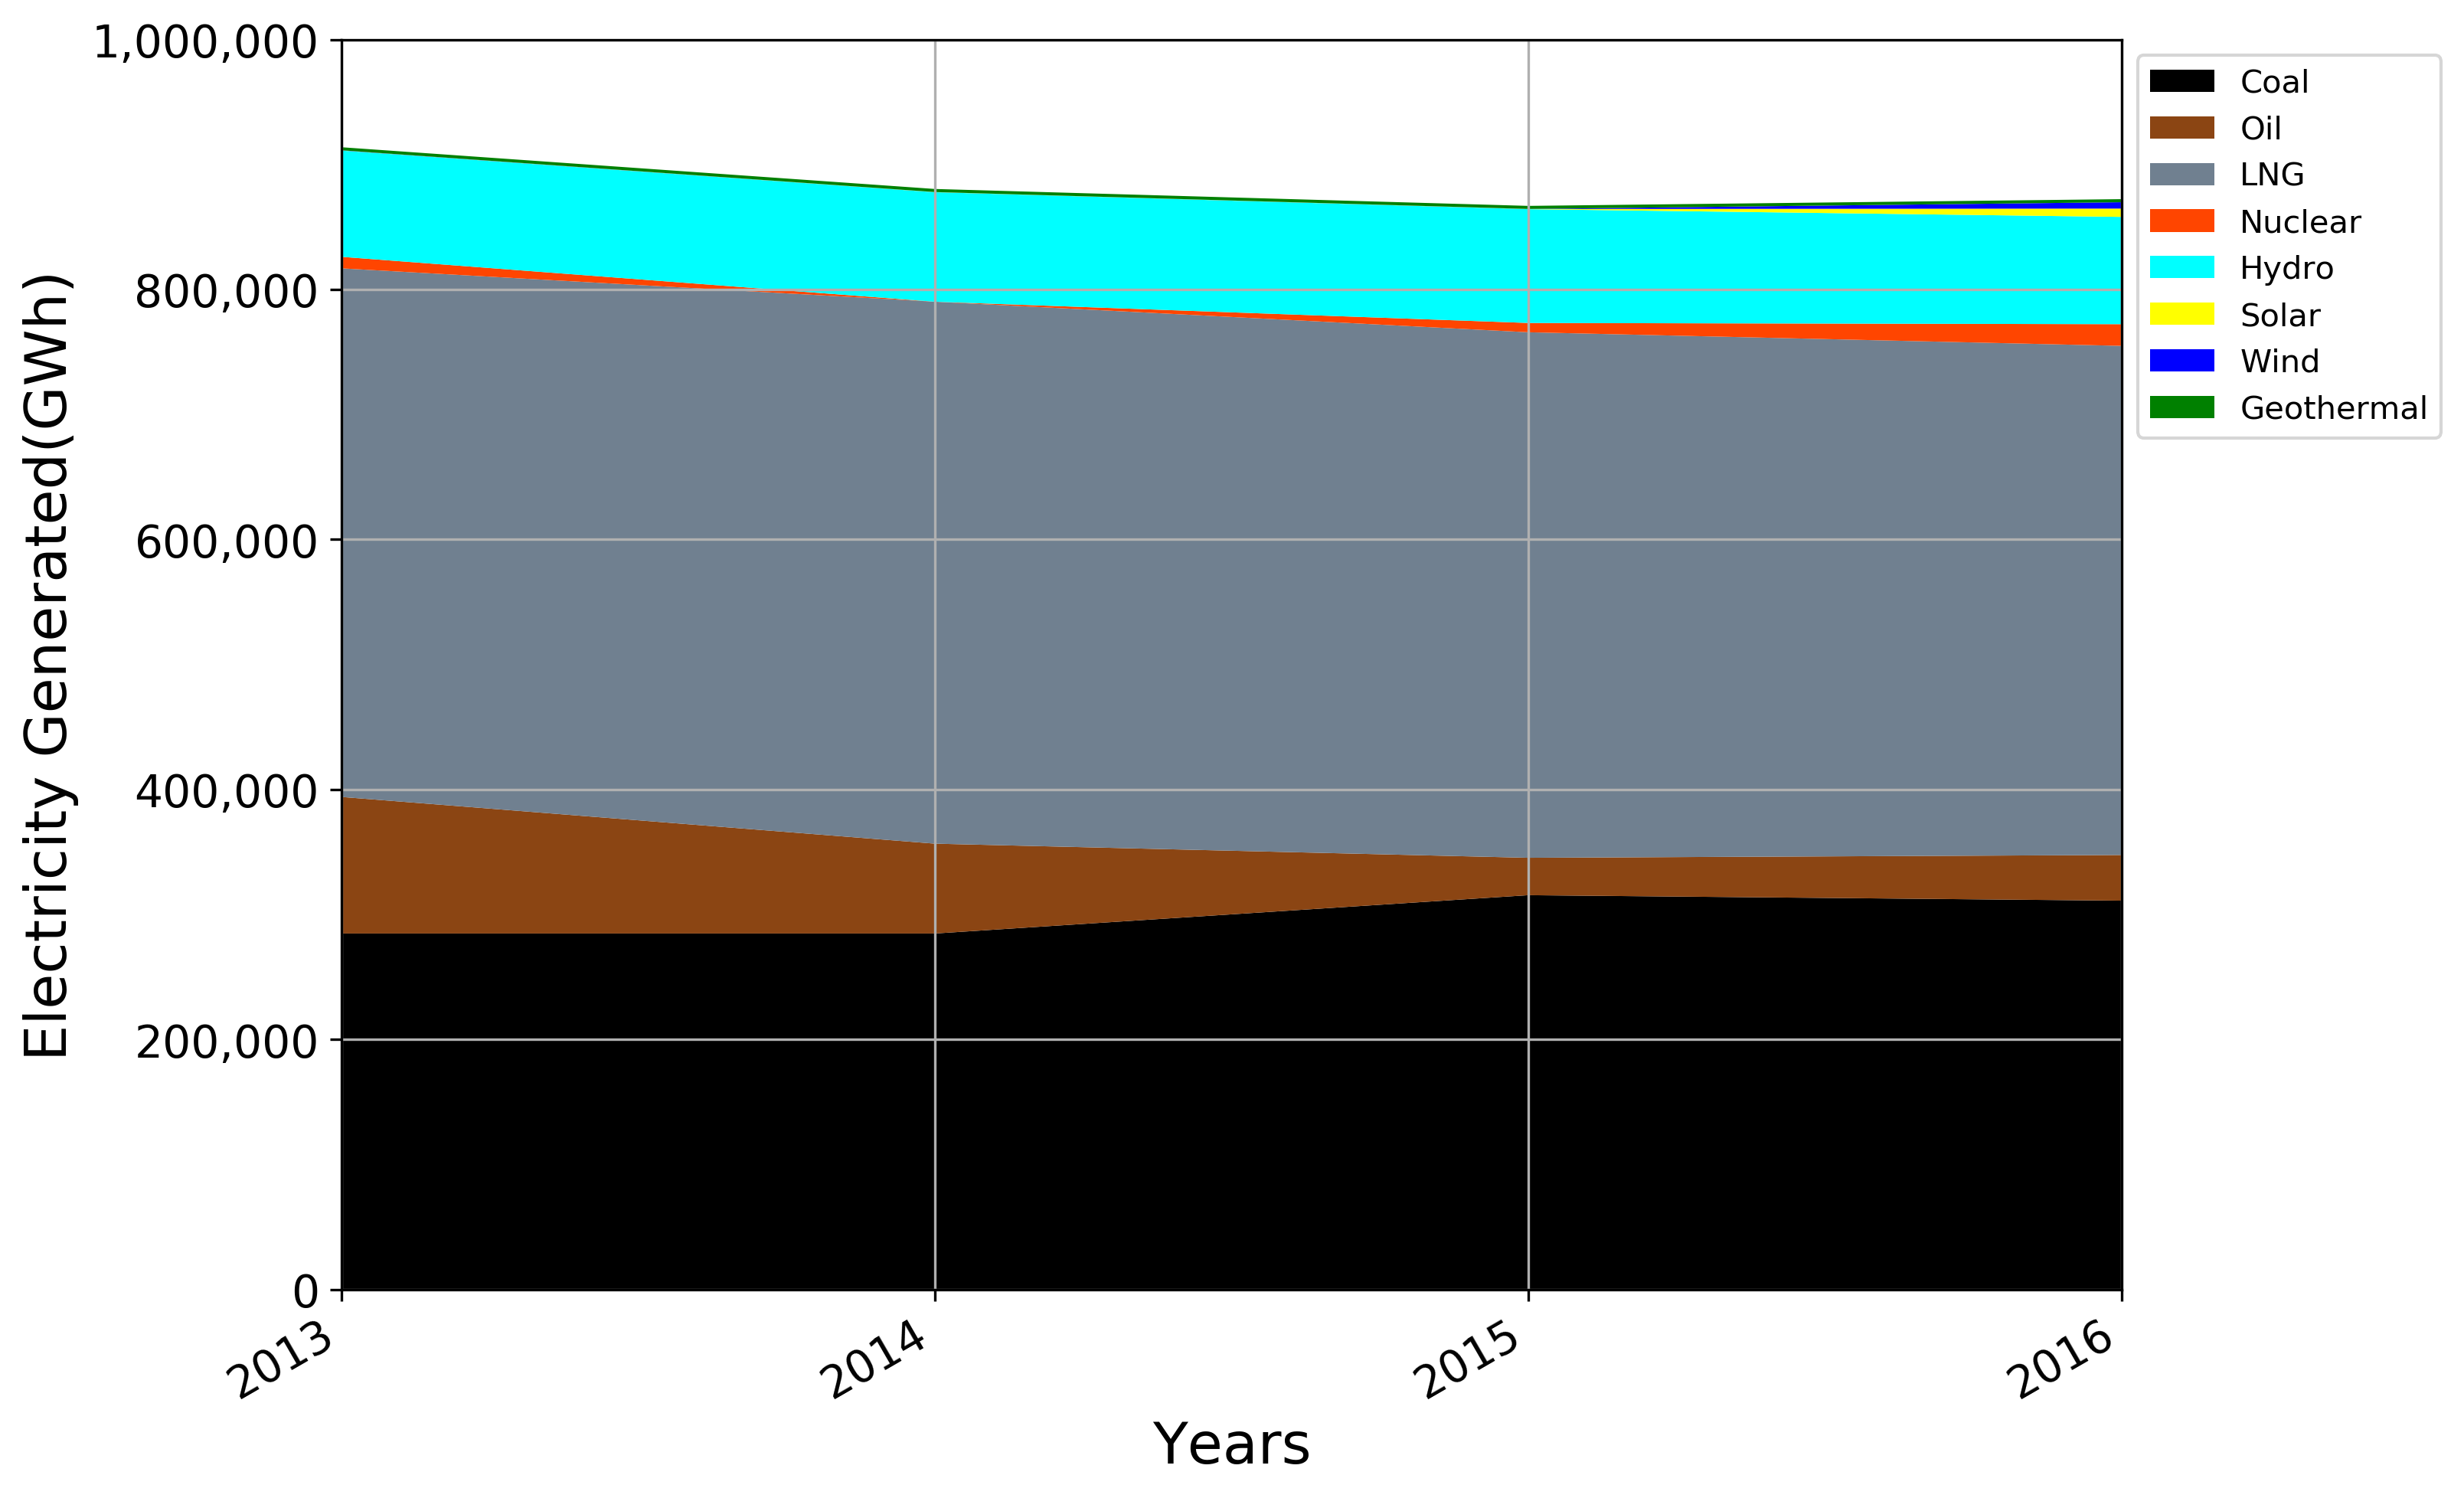
\includegraphics[scale=0.5]{figures/IC}
\caption{Electricity generation between 2013-2016 that defines the initial condition across all simulations.}
\end{figure}

\begin{table}[H]
\centering
	\caption{Initial condition for CO$_2$ emissions compared with data from the Carbon Brief\cite{carbonbrief_carbon_2018}.}
	\vspace{0.1in}
	\begin{tabularx}{0.55\textwidth}{p{0.05\textwidth} p{0.15\textwidth} p{0.15\textwidth} p{0.15\textwidth}}
		\hline
\textbf{Year} & \textbf{Model emissions} & \textbf{Actual emissions} & \textbf{Error} \\
  & (Mt CO$_2$-eq.) & (Mt CO$_2$-eq.) &  \\
\hline
2013 & 603.62 & 592.4 & 1.89 \% \\
2014 & 582.27 & 572.6 & 1.69 \% \\
2015 & 572.53 & 560.3 & 2.18 \% \\
2016 & 565.94 & 552.8 & 2.38 \% \\
\hline 
	\end{tabularx}
\label{ic-co2}
\end{table}

\begin{landscape}
\centering
\begin{longtable}{ |*{8}{c|} }
\caption{Economic data for modelled technologies.}\\
\hline
\textbf{Technology} & \textbf{Capital} & \textbf{Fixed} & \textbf{Variable} & \textbf{Lifespan} & \textbf{Capacity factor/} & \textbf{Emission} & \textbf{Year} \\
 & \textbf{cost} & \textbf{\gls{OM}} & \textbf{\gls{OM}} &  & \textbf{efficiency} & \textbf{coefficient} & \textbf{available} \\
 & (MUSD/GW) & (MUSD/GW) & (MUSD/GWh) & (Years)  &  & (gCO$_2$\added{-eq} /kWh)  &  \\
\hline
\endhead  % header material
\hline
\endfoot  % footer material
\hline
\endlastfoot
\gls{USC} \cite{eia_cost_2020,ipcc_climate_2014} & 3661 & 40.41 & 0.045 & 40 & CF=0.55 & 820 & 2017 \\
\gls{lng}\cite{eia_cost_2020,ipcc_climate_2014} & 1079 & 14 & 0.0025 & 30 & CF=0.55 & 490 & 2017 \\
Nuclear \cite{eia_cost_2020,ipcc_climate_2014,lokhov_load-following_2011} & 6317 & 121.13 & 2.36 & 60 & CF=0.6-0.95 & 12 & 2017 \\
Li-ion storage \cite{mongird_energy_2019,emilsson_lithium-ion_2019,oliveira_environmental_2015} & 1876 (2017) & 10 & 0.3 & 10 & Eff=0.86 & 151(2017) & 2017 \\
 & 1446 (2025) &  &  &  &  & 87(2050) &  \\
Solar \cite{eia_cost_2020,ipcc_climate_2014} & 1307(2017) & 15.19 & 0  & 25 & CF=0.14 & 37 & 2017 \\
 & 615(2050) & & & & & &  \\
Onshore wind & 3454(2017) & 136.37 & 0 & 25 & CF=0.25(2017) & 20(2017) & 2017 \\
\cite{eia_cost_2020,ipcc_climate_2014,kato_energy_2016,govindji_appraisal_2012,heger_wind_2016,bonou_life_2016} & 2406(2050) &  &  &  & CF=0.35(2050) & 7 (2040) &  \\
Offshore wind(Fixed) & 7772(2017) & 341 & 0 & 25 & CF=0.3(2017) & 25(2017) & 2017 \\
\cite{eia_cost_2020,ipcc_climate_2014,kato_energy_2016,govindji_appraisal_2012,heger_wind_2016,bonou_life_2016} & 3381(2050) &  &  & & CF=0.40(2050) & 11(2050) &  \\
Offshore wind(Floating) & 12897(2017) & 423 & 0 & 25 & CF=0.35(2017) & 25(2017) & 2017 \\
\cite{eia_cost_2020,ipcc_climate_2014,kato_energy_2016,govindji_appraisal_2012,heger_wind_2016,bonou_life_2016} & 5610(2050) &  &  &  & CF=0.45(2050) & 11(2050) &  \\
LNG-CCS(90\%) & 2626(2022) & 27.484 & 0.0494 & 30 & CF=0.12-0.4(2017) & 94 & 2022 \\
 \cite{eia_cost_2020,ipcc_climate_2014} & 1422(2050) &  & &  &  &  & \\
USC-CCS(90\%) & 5252(2023) & 59 & 0.078 & 40 & CF=0.27-0.32(2017) & 236.5 & 2023 \\
 \cite{eia_cost_2020,ipcc_climate_2014} & 4091(2050) &  &  &  &  &  & \\
Emerging Solar & 4600(2017) & 15.19 & 0 & 25 & Eff=0.22(2017) & 22(2017) & 2017 \\
 \cite{irena_solar_2012,peng_review_2013} & 600(2050) &  &  &  &Eff=0.3(2030)  & 13(2040) &  \\
\gls{AEC}  & 1500(2022) & 8 & 0.0004 & 11(CF=0.9) & Eff=0.7 & 1.29 & 2022\\
\cite{iea_technology_2015, bhandari_life_2014, cetinkaya_life_2012, burkhardt_hydrogen_2016} & 850(2030) &  &  &  &  & &  \\
\gls{PEMEC} & 3500(2022) & 8 & 0.0004 & 7 (2022)(CF=0.9) & Eff=0.75(2022) & 8.7(2022) & 2022\\
\cite{iea_technology_2015, bareis_life_2019, carmo_comprehensive_2013,ayers_research_2010,siracusano_influence_2017,schmidt_future_2017,mayyas_manufacturing_2019} & 1500(2030) &  & 11(2050)  &  & Eff=0.82(2030) & 0.456(2050)  &  \\
 & 400(2050) &  &  &  & &  &  \\
\gls{SOEC} & 6000(2030) & 8 & 0.0004 & 2 (2030)(CF=0.9) & Eff=0.9 & 5.4(2030) & 2030\\
\cite{iea_technology_2015,schmidt_future_2017,hafele_life_2016} & 1000(2050) &  &  & 7 (2050) &  & 1.08(2050) & \\
 & 400(2070) &  &  & 11 (2070) &  & 0.72(2070) & \\
Gas reforming  & 763 & 6.21 & 0.04 & 30  & Eff=0.7 & 356.6 & 2022\\
\cite{iea_technology_2015,mehmeti_life_2018,keipi_economic_2018} & & & & & &  & \\
Gas reforming-CCS(70\%) & 1200 & 8 & 0.065 & 30 & Eff=0.56 & 179 & 2022\\
\cite{iea_technology_2015,keipi_economic_2018,cormos_ana-maria_economic_2018} &  &  &  &  &  &  & \\
\gls{PEMFC} \cite{iea_technology_2015,simons_life-cycle_2015,kannan_life_2007} & 7399(2022) & 30.65 & 0.59 & 7 (CF=0.9) & Eff=0.49 & 1.087(2022) & 2022\\
 & 4000(2030) &  &  &  &  & 0.65(2030) &  \\
 & 3000(2035) &  &  &  &  &  &  \\
\gls{SOFC} \cite{iea_technology_2015,simons_life-cycle_2015,rillo_life_2017,tu_advances_2004} & 7399(2030) & 30.65 & 0.59 & 10 (CF=0.9) & Eff=0.7 & 2.11(2030) & 2030\\
 & 4000(2035) &  &  &  &  & 1.27(2040) &  \\
 & 3000(2040) &  &  &  &  & &  \\
\gls{PWS} \cite{pinaud_technical_2013} & 14706  & 236.5 & 0 & 20(CF=0.9) & Eff=0.15(2050) & Unknown & 2050
\label{eco}
\end{longtable}
\end{landscape}



\begin{table}[H]
\centering
	\caption{Nameplate capacity deployment limits.}
	\vspace{0.1in}
	\begin{tabularx}{0.7\textwidth}{p{0.35\textwidth} p{0.35\textwidth} }
		\hline
\textbf{Technology} & \textbf{Net Capacity} \textbf{Limit} (GW)\\
\hline
Photovoltaic \cite{isep_53_2018} & 332 \\
Onshore wind \cite{heger_wind_2016,kato_energy_2016} & 180 \\
Offshore wind (fixed) \cite{heger_wind_2016,kato_energy_2016}& 130 \\
Offshore wind (floating) \cite{heger_wind_2016,kato_energy_2016}& 260 \\
Nuclear & 50 (Scenarios 3 \& 4) \\
 & 100 (Scenario 2) \\
\gls{PWS} \cite{pinaud_technical_2013} & 100 (Scenario 5) \\
\hline 
\end{tabularx}
\label{caplim}
\end{table}

\begin{table}[H]
\centering
%\begin{minipage}{\textwidth} 
	\caption{Nameplate capacity growth rates.}
	\vspace{0.1in}
	\begin{tabularx}{0.8\textwidth}{p{0.35\textwidth} p{0.45\textwidth}}
		\hline
\textbf{Technology} & \textbf{Maximum Annual Growth Rate} \\
%  & \textbf{Growth Rate}   \\
\hline
Nuclear (2027 onwards) & +5 reactors \\
Solar and emerging solar \cite{irena_renewable_2020} & 40\%  \\
Onshore wind \cite{irena_renewable_2020} & 25\% \\
Offshore wind(Fixed) \cite{irena_renewable_2020} & 20\% \\
Offshore wind(Floating) \cite{irena_renewable_2020} & 20\% \\
Li-ion storage & 30\% \\
Natural gas &  50\% \\
\gls{USC} & 50\% \\
All emerging technologies & 40\% (Years 1-5) \\
& 60\% (Years 6-10) \\
 & 40\% (Years 11-15) \\
 & 30\% (Years 16-) \\
\hline 
\end{tabularx}
\label{growrate}
%\end{minipage}
\end{table}

\begin{table}[H]
\centering
	\caption{Miscellaneous model parameters and assumptions.}
	\vspace{0.1in}
	\begin{tabularx}{0.5\textwidth}{p{0.3\textwidth} p{0.2\textwidth}}
		\hline
\textbf{Parameter} & \textbf{Value} \\
\hline
Currency & MUSD 2015 \\
Activity unit & GWh\\
Discount rate & 5\% \\
Transmission efficiency & 90 \% \\
Li-ion discharge time \cite{mongird_energy_2019} & 4h \\
Li-ion E/P ratio \cite{mongird_energy_2019} & 4  \\
Li-ion depth-of-discharge \cite{mongird_energy_2019} & 80\% \\
Li-ion lifetime cycles \cite{mongird_energy_2019} & 3500  \\
\hline 
	\end{tabularx}
\label{misc-assump}
\end{table}

\pagebreak 

\section{Sensitivity analysis secondary results}

\begin{figure}[H] 
\centering
\hspace*{-1cm}
\includegraphics[scale=0.09]{figures/pws}
\caption{Sensitivity analysis of Photochemical Water Splitting. Red dots indicate points that are zero values, while blue dots indicate non-zero values.}
\label{pws}
\end{figure}

\begin{figure}[H] 
\centering
%\hspace*{-3cm}
\includegraphics[scale=0.12]{figures/satechsh2}
\caption{Sensitivity analysis of hydrogen generation technologies \gls{SOEC} and \gls{PEMEC}}.
\label{satechs-h2}
\end{figure}

\begin{figure}[H] 
\centering
%\hspace*{-3cm}
\includegraphics[scale=0.12]{figures/satechselc}
\caption{Sensitivity analysis of electricity generation technologies \gls{SOFC} and \gls{CCS} gas.}
\label{satechs-elc}
\end{figure}


\begin{figure}[H] 
\centering
%\hspace*{-3cm}

\includegraphics[scale=0.15]{figures/syscost}
\caption{Sensitivity analysis of the model's overall transition cost between 2013-2100 with respect to selected model parameters.}
\label{syscost}
\end{figure}

\begin{figure}[h] 
\centering
\hspace*{-3cm}
\includegraphics[scale=0.07]{figures/useless}
\caption{Sensitivity analysis results for \gls{PEMFC} and \gls{CCS} coal.}
\label{sa-useless}

\end{figure}
\end{document}
